%% LyX 2.0.7 created this file.  For more info, see http://www.lyx.org/.
%% Do not edit unless you really know what you are doing.
\documentclass[english,msc,oneside]{ubcthesis}
\usepackage{mathptmx}
\usepackage{helvet}
\renewcommand{\ttdefault}{cmtt}
\renewcommand{\familydefault}{\rmdefault}
\usepackage[T1]{fontenc}
\setcounter{tocdepth}{1}
\usepackage{array}
\usepackage{verbatim}
\usepackage{float}
\usepackage{fancybox}
\usepackage{calc}
\usepackage{amsthm}
\usepackage{amsmath}
\usepackage{graphicx}
\usepackage[authoryear]{natbib}

\makeatletter

%%%%%%%%%%%%%%%%%%%%%%%%%%%%%% LyX specific LaTeX commands.
%% Because html converters don't know tabularnewline
\providecommand{\tabularnewline}{\\}

%%%%%%%%%%%%%%%%%%%%%%%%%%%%%% User specified LaTeX commands.

\usepackage{afterpage}

\usepackage{float}

%\usepackage{alltt}

\usepackage{longtable}

\usepackage{graphicx}

\usepackage{lscape}

%\usepackage[numbers,sort&compress]{natbib}

\usepackage{psfrag}

\usepackage{listings}
\usepackage{minted}
\usepackage{placeins}

%\usepackage[hypertex,final=true,unicode=true, pdfusetitle,bookmarks=true,bookmarksnumbered=false,bookmarksopen=true,breaklinks=true,pdfborder={0 0 1},backref=true,colorlinks=true,citecolor=black, filecolor=black, linkcolor=black, urlcolor=black]{hyperref}
\usepackage{hyperref}
\hypersetup{
hypertex=true,
unicode=true, pdfusetitle,
bookmarks=true,
bookmarksnumbered=false,
bookmarksopen=true,
breaklinks=true,
pdfborder={0 0 1},
backref=true,
colorlinks=true,
citecolor=black,
filecolor=black,
linkcolor=black,
urlcolor=black
}

% These commands are optional.  The defaults are shown.  You only
% need to include them if you need a different value
\institution{The University Of British Columbia}

% If you are at the Okanagan campus, then you should specify these
% instead.
%\faculty{The College of Graduate Studies}
%\institutionaddress{Okanagan}
\faculty{The Faculty of Graduate Studies}
\institutionaddress{Vancouver}

% You can issue as many of these as you have...
\previousdegree{B.E, University of Pune, 2006}

% You can override the option setting here.
% \degreetitle{Jack of All Trades}

% These commands are required.
\title{Advances in password cracking and reverse engineering}
\author{Dhirendra Singh Kholia}
\copyrightyear{2013}
\submitdate{\today}

\program{Computer Science}

% These commands are presently not required for UBC theses as the
% advisor's name and title are not presently required anywhere.
%\advisor{Ariel R.~Zhitnitsky}
%\advisortitle{Professor of Physics}

% One might want to override the format of the section and chapter
% numbers.  This shows you how to do it.  Note that the current
% format is acceptable for submission to the FoGS: If you wish to modify
% these, you should check with the FoGS explicity. prior to making
% the modifications.
\renewcommand\thepart         {\Roman{part}}
\renewcommand\thechapter      {\arabic{chapter}}
\renewcommand\thesection      {\thechapter.\arabic{section}}
\renewcommand\thesubsection   {\thesection.\arabic{subsection}}
\renewcommand\thesubsubsection{\thesubsection.\arabic{subsubsection}}
\renewcommand\theparagraph    {\thesubsubsection.\arabic{paragraph}}
\renewcommand\thesubparagraph {\theparagraph.\arabic{subparagraph}}

% Following now set in LyX
%\setcounter{tocdepth}{2}
%\setcounter{secnumdepth}{2}

% Here is an example of a "Program" environment defined with the
% "float" package.  The list of programs will be stored in the file
% ubcsample.lop and the numbering will start with the chapter
% number.  The style will be "ruled".
\floatstyle{ruled}
\newfloat{Program}{htbp}{lop}[chapter]

\makeatother

\usepackage{babel}
\usepackage{xunicode}
\begin{document}
\frontmatter
\maketitle
\begin{abstract}
This paper presents recent advances in the areas of password cracking
and reverse engineering. In particular, it describes the design and
implementation of various plug-ins for John the Ripper \citep{Peslyak:1996},
Ettercap \citep{ALoR:2001}, Nmap \citep{Fyodor:1997} and Metasploit
Framework \citep{Moore:2003} for mounting attacks against various
password protected file formats, password managers, authentication
protocols and hashed passwords. 

Chapter \ref{chap:backup-solutions} presents the security analysis
of various cloud backup solutions (Dropbox, inSync Druva). Chapter
\ref{chap:file-formats} presents security analysis of various file
formats (called ``non-hashes'') and password managers. Chapter \ref{chap:auth-protocols}
presents security analysis of various authentication protocols. Security
analysis of various password hashing algorithms is covered in Chapter
\ref{chap:hashes-JtR}. 

One of the motivation behind this work is to build open-source security
tools which can compete with offerings from commercial companies like
Elcomsoft and Passware, who are well known in the field of password
recovery. Our work describes various JtR plug-ins offering new functionality
which is not available even in existing commercial password recovery
softwares. Some of our plug-ins are even faster and more scalable
than the ones available commercially.
\end{abstract}
\tableofcontents{}

\listoftables
\listoffigures
\listof{Program}{List of Programs}


\chapter{Acknowledgements}

This is the place to thank professional colleagues and people who
have given you the most help during the course of your graduate work. 

I would like to thanks Solar Designer for mentoring my GSoC 2011 (Google
Summer of Code) work, Robert for collaborating on Mac OS X Keychain
work, Lukas for GPU implementation of Password Safe format, Nigel
for collaborating on RACF work, magnum for maintaing JtR-jumbo, Milen
for collaborating on FileVault work.

XXX use more words than code

XXX improve graphs, use gnuplot


\chapter{Dedication}

This thesis is dedicated to the entire john-users and john-dev community.
Special thanks goes to Solar Designer, magnum and Jim Foug.


\chapter{Statement of Co-Authorship}

While this thesis is authored solely, I was assisted in my research
by the following people (and their work).
\begin{itemize}
\item Solar Designer (overall mentorship)
\item RACF hashing format (Nigel Pentland (author of CRACF) and Phil Young).
\item Apple DMG file format (Milen Rangelov)
\item Apple Keychain format (Matt Johnson)
\item 1Password file format (XXX)
\end{itemize}
	
\mainmatter


% Parts are the largest structural units, but are optional.
%\part{Thesis}
% Chapters are the next main unit.




\chapter{Analysis of security of various file formats.\label{chap:file-formats}}

This section presents analysis of various file formats and programs
which allow encryption of user data from a cracking perspective. A
note about benchmarking, AMD FX-8120 is not a true 8-core CPU and
use dynamic frequency scaling, hence the practical speedups obtained
by using all 8 cores will be less than 8x. The maximum speedup factor
of AMD FX-8120 is (3.1 GHz / 4 GHz) {*} 8 = 6x when using all 8 cores.
Almost all the JtR plug-ins described in this paper are multi-core
(by using OpenMP) as well as multi-node (by using MPI). Some of the
plug-ins are also implemented in OpenCL resulting in speed-ups of
over 150x.


\section{Password Safe 3.x }

Password Safe \citep{Schneier:2002} is a free and open source software
program for storing passwords originally authored by Bruce Schneier.
From a developer point of view, this format has been easiest to write
cracking code for since the database format is well documented in
formatV3.txt file \citep{Shapiro:2003} and \citep{Hinegardner:2007}.
The same database format is used by Password Gorilla \citep{Pilhofer:2006}
as well as Pasaffe password manager \citep{Deslauriers:2011}, so
the analysis here applies to them too. See \citep{Hinegardner:2007}
for more details on the database format and encryption / decryption
process. Table \ref{tab:pwsafe} describes the fields present in Password
Safe database.

\begin{table}[h]
%optional [t, b or h];
 

\begin{tabular}{|>{\raggedright}m{2cm}|>{\raggedright}m{1.5cm}|>{\raggedright}m{8cm}|}
\hline 
TAG & 4 bytes & The 4 ASCII Characters ‘PWS3’\tabularnewline
\hline 
SALT & 32 bytes & 256 random bit value generated at file creation\tabularnewline
\hline 
ITER & 32 bit LE value & number of rounds in the key stretch algorithm\tabularnewline
\hline 
H(P’) aka HASH & 32 bytes & SHA-256 of the user’s ``processed'' passphrase\tabularnewline
\hline 
B1 & 16 bytes & Encrypted 128 random value using P’ with Twofish algorithm\tabularnewline
\hline 
B2 & 16 bytes & Encrypted 128 random value using P’ with Twofish algorithm\tabularnewline
\hline 
B3 & 16 bytes & Encrypted 128 random value using P’ with Twofish algorithm\tabularnewline
\hline 
B4 & 16 bytes & Encrypted 128 random value using P’ with Twofish algorithm\tabularnewline
\hline 
Init vector & 16 bytes & 128 bit random Initialization Vector for the content’s encryption\tabularnewline
\hline 
Header & 16 bytes & General information for the database \tabularnewline
\hline 
Records & 16 bytes & The records in the database\tabularnewline
\hline 
EOF  & 16 bytes & unencrypted string “PWS3-EOFPWS3-EOF” \tabularnewline
\hline 
HMAC & 32 bytes & 256 bit SHA-256 hash of the plaintext contents, starting with the
version number in the header and ending with the last field of the
last record\tabularnewline
\hline 
\end{tabular}

\caption{\label{tab:pwsafe} Password Safe 3 database format (header fields,
in order)}
\end{table}


From a cracking perspective, only SALT, ITER and H(P') fields are
needed. The Password Safe 3 format uses \textquotedbl{}variable key
stretching\textquotedbl{} to protect a database against brute-force
attacks. The higher the value of \textquotedbl{}iterations\textquotedbl{}
(ITER) parameter is, the longer it to test a candidate password. The
Password Safe 3 format avoids a potential weakness discovered with
the old Password Safe 2 (\textquotedbl{}V2\textquotedbl{}) file format
which allowed brute force attacks 1000 times faster than intended.
The Password Safe 3 format avoids this issue by depending on the result
of the key stretching operation and using it as an input for decryption
of data. The key stretching algorithm used in Password Safe is described
in Program is \ref{prog:psc}. For full implementation details see
\textit{src/pwsafe2john.c} and \textit{src/pwsafe\_fmt\_plug.c}.

\begin{Program}[h]
\caption{\label{prog:psc}Password Safe Cracker
}
\vspace{0.4cm}

\begin{minted}[linenos=false]{c}

SHA256_CTX ctx;

SHA256_Init(&ctx);
SHA256_Update(&ctx, password, strlen(password);
SHA256_Update(&ctx, SALT, 32);
SHA256_Final(output, &ctx);

for(int i = 0; i <= ITER; i++)  {
	SHA256_Init(&ctx);
	SHA256_Update(&ctx, output, 32);
	SHA256_Final(output, &ctx);
}

if(output == HASH) {
	/* password cracked */
}
\end{minted}
\end{Program}

Our CPU version of the cracking software achieves around 896 c/s on
a single core and 7097 c/s on 2 x Xeon E5420 (8 cores total). The
GPU version (authored by Lukas Odzioba based on our CPU implementation)
achieves a speedup of around 89x over single core CPU result. Currently,
the GPU implementation transfers candidate passwords from CPU to GPU
which is sub-optimal. Future version of JtR will remove this limitation
and higher cracking speeds can be expected. 

\begin{figure}[h]
\includegraphics[scale=0.75]{\string"resources/Password Safe Benchmarks\string".png}

\caption{Password Safe Cracking Benchmarks}
\end{figure}


\vspace{0.4cm}

\begin{Program}
\caption{\label{prog:fib}Password Safe Benchmarks
}

\renewcommand{\lstlistingname}{Code}
\lstset{tabsize=2,basicstyle=\ttfamily,breaklines=true,columns=flexible,xleftmargin=1pt}
\lstinputlisting[language=C]{resources/pwsafe_output.txt}
\end{Program}

\FloatBarrier

Password Safe doesn't support the use of \textquotedbl{}Key Files\textquotedbl{}
(described in \citep{Reichl:2003}) . However, for added security,
YubiKey hardware \citep{Ehrensvrd:2007} which provides 2-Factor Authentication
can be used with Password Safe program. So far, no vulnerabilities
have been been published for the YubiKey device. Also, it is trivial
to increase resistance against brute-force attacks by simply increasing
the value of ITER field


\section{Apple Mac OS X Keychain }

Apple's keychain is a password management system in Mac OS. Keychain
software is an integral part of Mac OS since Mac OS 8.6. In Mac OS
X, keychain files are stored in \textasciitilde{}/Library/Keychains/,
/Library/Keychains/, and /Network/Library/Keychains. The default keychain
file is the login keychain (which all users have), typically unlocked
on login by the user's login password (blurb borrowed from \citet{Misc:1999}).

Keychain is an open-source software but compiling modern versions
of it on modern Mac OS systems is next to impossible (The whole OpenDarwin
project was abandoned in 2006 and the new PureDarwin project has been
unable to build security subsystem). Some of the bits required to
build Keychain haven't been released as open-source further complicating
the compilation process. In addition, Apple's own documentation regarding
Keychain's file format \citet{Apple:2004} is bogus. All these points
lead us to doubt the usefulness of Apple's open-source strategy.

Our JtR plug-in and security analysis of Mac OS X Keychain is an extension
of the original research done by Matt Johnston (author of extractkeychain
program \citep{Johnston:2004}). Table \ref{tab:keychain} describes
the file format uses by Apple's Keychain software.

\begin{table}[H]
%optional [t, b or h];
 %
\begin{tabular}{|c|c|c|>{\centering}p{5.5cm}|}
\hline 
Offset & Length & Name & Purpose\tabularnewline
\hline 
\hline 
0 & 4 bytes & Magic Number & Identify Keychain files\tabularnewline
\hline 
4 & 4 bytes & Version & Identify Keychain version \tabularnewline
\hline 
8 & 4 bytes & crypto-offset & offset of the encryption and signing key (length 48)\tabularnewline
\hline 
12 & 4 bytes & total length & total length of the keychain\tabularnewline
\hline 
16 & 16 bytes & signature & -\tabularnewline
\hline 
32 & 4 bytes & sequence & -\tabularnewline
\hline 
36 & 4 bytes & idle timeout & Idle time after which the Keychain is locked automatically\tabularnewline
\hline 
40 & 4 bytes & lock on sleep flag & -\tabularnewline
\hline 
44 & 20 bytes & SALT & Salt for PKBDF2\tabularnewline
\hline 
64 & 8 bytes & IV  & Initialization vector for 3DES-EDE\tabularnewline
\hline 
72 & 20 bytes & Blob Signature & Checksum of the blob\tabularnewline
\hline 
crypto-offset & 48 bytes & Ciphertext Data & encryption and signing key (length 48)\tabularnewline
\hline 
\end{tabular}

\caption{\label{tab:keychain} Apple Keychain file format (DbBlob)}
\end{table}


Mac OS X Keychain Services API provides functions to perform most
of the Keychain operations needed by applications. By using the SecKeychainUnlock
function exposed by the mentioned API, it is trivial to create a small
bruteforce attack program. An example of such a cracker is shown in
Program \ref{prog:keychain}. 

\begin{Program}[h]
\caption{\label{prog:keychain}Keychain Trivial Cracker
}
\vspace{0.2cm}

\begin{minted}[linenos=false]{c}
#include <Security/SecKeychain.h>

int main(void)
{
  OSStatus err;
  char passphrase[128];

  /* attack default keychain */
  SecKeychainRef keychain = NULL;
 
  /* argv[1] contains target keychain's name */
  while(fgets(passphrase, 128, stdin) != NULL) {
    err = SecKeychainUnlock(keychain,
      strlen(password), password, TRUE);
    if (!err) {
      printf ("Password Found : %s\n", password);
      exit(0);
    }
  }
}
\end{minted}
\end{Program}

However, such programs are capable of running only on Mac OS systems.
In addition, the cracking speed of such programs is typically limited
to < 500 passwords per second on modern processors and it is not possible
to take advantage of multiple cores due to single-threaded nature
of securityd. To overcome these limitations, we have build a custom
multi-core cross-platform cracking software for Mac OS X Keychain. 

The interesting parts of the Keychain are called \textquotedbl{}blobs\textquotedbl{}
(see \citep{Johnston:2004}) and there are two types of blobs: database
blobs and key blobs. There’s only one DbBlob (at the end of the file),
and that contains the file encryption key (amongst other things),
encrypted with the master key. The master key is derived purely from
the user’s password, and a salt, also found in the DbBlob. PKCS \#5
v2.0 PBKDF2 \citep{kaliski2000pkcs:2000} is used for deriving the
master key. The Mac OS X keychain uses the HMAC-SHA-1 function with
1000 iterations, a salt length of 20 bytes and intended length of
24 bytes. In other words, Master Key = PBKDF2-HMAC-SHA(PASSWORD, SALT,
1000, 24). This master key is used to decrypt the encrypted file encryption
key. The Mac OS X keychain uses CMS padding \citep{housley1999cryptographic:1999}
for wrapping the file encryption key. The original un-encrypted file
encryption key material has length equal to 44 bytes which is padded
to 48 bytes before 3DES encryption. We exploit this padding knowledge
to figure out if we have successfully decrypted the encrypted file
encryption key. We do not know of any other existing research work
which uses this technique. The key steps involved are shown in Program
\ref{prog:keychainpro}.

\begin{Program}[h]
\caption{\label{prog:keychainpro}Keychain Cracker
}
\vspace{0.2cm}

\begin{minted}[linenos=false]{c}
/* CIPHERTEXT is encrypted file encryption key */

/* generate encryption key */
unsigned int master[8];
pbkdf2(PASSWORD,  strlen(PASSWORD), SALT, \
  SALTLEN, 1000, master);

DES_cblock key1, key2, key3;
DES_cblock ivec;
DES_key_schedule ks1, ks2, ks3;
memcpy(key1, key, 8);
memcpy(key2, key + 8, 8);
memcpy(key3, key + 16, 8);
DES_set_key((C_Block *) key1, &ks1);
DES_set_key((C_Block *) key2, &ks2);
DES_set_key((C_Block *) key3, &ks3);
memcpy(ivec, IV, 8);
DES_ede3_cbc_encrypt(CIPHERTEXT, out, 48, \
   &ks1, &ks2, &ks3, &ivec,  DES_DECRYPT);

// now check padding
pad = out[47];
if(pad > 8)
   // "Bad padding byte. Wrong Password.
   return -1;
if(pad != 4) 
   // "Bad padding value. Wrong Password.
   return -1;
n = CTLEN - pad;
for(i = n; i < CTLEN; i++)
   if(out[i] != pad)
      // "Bad padding. Wrong Password.
   return -1;

// padding check passed, password found!
printf("Password Found");
\end{minted}
\end{Program}

For full implementation details see \textit{src/keychain2john.c},
\textit{src/keychain\_fmt\_plug.c} and \textit{src/opencl\_keychain\_fmt.c}
files. The algorithms used in our JtR plug-in have been verified by
Robert Vežnaver in his master's thesis \citep{VeÅŸnaver:2012}.

Our initial GPU implementation which does PBKDF2 operations on GPU
and 3DES operations on multiple-cores is roughly 332X faster than
the single-core AMD X3 720 CPU results. 

\begin{figure}[h]
\includegraphics[scale=0.75]{\string"resources/Keychain Benchmarks\string".png}

\caption{Keychain Cracking Benchmarks}
\end{figure}


\vspace{0.4cm}

\begin{Program}[h]
\caption{\label{prog:keychainout}OSX Keychain Benchmarks
}

\renewcommand{\lstlistingname}{Code}
\lstset{tabsize=2,basicstyle=\ttfamily,breaklines=true,columns=flexible,xleftmargin=1pt}
\lstinputlisting[language=C]{resources/keychain_output.txt}
\end{Program}

\FloatBarrier

In our opinion, the default number of iterations (1, 000) should be
increased for added security against brute-force attacks. However,
the current file format used by Keychain does not provide a way to
do so without breaking compatibility with existing Mac OS systems.
Our cracker is the fastest as well as the only GPU based cracker for
Mac OS Keychain files.


\section{1Password Keychains (Cloud and Agile Keychains) }

1Password is a popular password manager available for Windows, iPad,
iPhone, Android and Mac platforms. 1Password supports two file formats
(called Agile Keychain and Cloud Keychain) which is different from
Apple's Keychain file format. The goal of the Agile Keychain file
is to build on the successes of the Mac OS X keychain while increasing
the flexibility and portability of the keychain design (\citet{AgileBits:2008}
and \citet{AgileBits:2012}) . 1Password stores its data in a folder
called ``1Password.agilekeychain''. 1Password uses JSON (JavaScript
Object Notation) format to store its data which has a benefit that
its files can be loaded directly into a web browser. It is possible
to access the data, without installing 1Password software , by using
a web browser. Our JtR plug-in and security analysis of Agile Keychain
is an extension of the original research done by Antonin Amand (author
of agilekeychain, see \citep{Amand:2009})

The core of the encryption is AES (Advanced Encryption Standard) using
128-bit encryption keys and performed in Cipher Block Chaining (CBC)
mode along with a randomized Initialization Vector. Instead of encrypting
data with the password directly, a random key of 1024 bytes is used.
This key is stored in the encryptionKeys.js file, encrypted using
a key derived from the users master password by using PBKDF2 function.
A sample encryptionKeys.js is shown in Program \ref{prog:agilekeychain}.

\begin{Program}[H]
\caption{\label{prog:agilekeychain}Sample encryptionKeys.js
}
\vspace{0.2cm}

\begin{minted}[linenos=false]{js}
{
    "list": [
        {
            "data": "U2FsdGVkX19xRuqhzKOV5efr...",
            "validation": "U2FsdGVkX19dIEp7VK09LOf...",
            "identifier": "1D169F66FAAC4745A4C708B254944791",
            "iterations": 1000
        }
    ]

    SALT = identifier value
    User_Encryption_Key = PBKDF2-HMAC-SHA(PASSWORD, \
        SALT, iterations, 16)
}
\end{minted}
\end{Program}

We have written a Python program \textit{(run/agilekc2john.py}) which
parses Agile Keychain data and generates a ``hash'' which is understood
by JtR. 1Password uses PKCS\#7 padding\citep{kaliski1998pkcs} for
wrapping the random encryption key. We exploit this padding knowledge
to figure out if we have successfully decrypted the random encryption
key.

\begin{figure}[H]
\caption{Agile Keychain Benchmarks}


\includegraphics[scale=0.75]{\string"resources/Agile Keychain Benchmarks\string".png}
\end{figure}


\begin{Program}[H]
\caption{\label{prog:agilekeychaincracker}Agile Keychain Cracker
}
\vspace{0.2cm}

\begin{minted}[linenos=false]{c}
/* CIPHERTEXT is encrypted random key */

#define CTLEN 1040

unsigned int master[8];
pbkdf2(PASSWORD, strlen(PASSWORD), SALT, SALTLEN, iters, master);
AES_KEY akey;
AES_set_decrypt_key(master, 128, &akey);
AES_cbc_encrypt(CIPHERTEXT, out, CTLEN, &akey, iv, AES_DECRYPT);

// now check padding
pad = out[CTLEN - 1];
if(pad < 1 || pad > 16) /* AES block size is 128 bits = 16 bytes */
   // "Bad padding byte. You probably have a wrong password"
   return -1;

n = CTLEN - pad;
key_size = n / 8;

if(key_size != 128 && key_size != 192 && key_size != 256)
   // "invalid key size"
   return -1;
for(i = n; i < CTLEN; i++)
   if(out[i] != pad)
      // "Bad padding. You probably have a wrong password"
      return -1;

// padding check passed, password found!
printf("Password Found");
\end{minted}
\end{Program}

\begin{Program}
\caption{\label{prog:fib}Agile Keychain Benchmarks
}

\renewcommand{\lstlistingname}{Code}
\lstset{tabsize=2,basicstyle=\ttfamily,breaklines=true,columns=flexible,xleftmargin=1pt}
\lstinputlisting[language=C]{resources/agilekeychain_output.txt}
\end{Program}

\FloatBarrier

In our opinion, the default number of iterations (1,000) should be
increased for added security against brute-force attacks. It is trivial
to do so by increasing the value of ``iterations'' parameter in
encryptionKey.ks file. However doing this on mobile platforms might
have an adverse impace on responsiveness and usability. Our cracker
is the only known cracker for Agile Keychain files. Agile Keychain
design has one flaw that it doesn't encrypt and protect the metadata
(like URL) for a given password. This opens up another attack vector
against 1Password software.

\begin{Program}
\caption{\label{prog:fib}Agile Keychain metadata flaw
}

\renewcommand{\lstlistingname}{Code}
\lstset{tabsize=2,basicstyle=\ttfamily,breaklines=true,columns=flexible,xleftmargin=1pt}
\lstinputlisting{resources/agilekeychain_metadata.txt}
\end{Program}

It was interesting to see our cracker being tested and blogged about
by official 1Password developer Jeffrey Goldberg \citep{Goldberg:2012}.


\section{GNOME Keyring }

GNOME Keyring is a collection of components in GNOME that store secrets,
passwords, keys, certificates and make them available to applications.
GNOME Keyring is integrated with the user's login, so that their secret
storage can be unlocked when the user logins into their session. GNOME
Keyring is a daemon application designed to take care of the user's
security credentials, such as user names and passwords. The sensitive
data is encrypted and stored in a keyring file in the user's home
folder (in \textasciitilde{}/.gnome2/keyrings folder) and have ``keyring''
extension. The default keyring uses the login password for encryption,
so users don't need to remember yet another password \citep{GnomeKeyring}.

GNOME Keyring is implemented as a daemon and uses the process name
gnome-keyring-daemon. Applications can store and request passwords
by using the libgnome-keyring library. GNOME Keyring is used by various
applications like Firefox, Chromium and SSH to stores credentials.

Our program gkcrack \citep{kholia:2012} is the only program that
can crack password protected GNOME Keyrings. However, gkcrack program
is not a multi-core capable API due to the gnome-keyring-daemon being
single threaded. Besides, gkcrack requires GNOME Keyring daemon to
be running and also keyring files must be accessible to the daemon.
Program \ref{prog:keyring-trivial} shows the sketch of gkcrack program.

\begin{Program}[H]
\caption{\label{prog:keyring-trivial}Trivial GNOME Keyring cracker
}
\vspace{0.2cm}

\begin{minted}[linenos=false]{c}
#include <gnome-keyring.h>
#include <stdio.h>

int main(int argc, char **argv)
{
   char passphrase[128];
   GnomeKeyringResult r;

    /* argv[1] contains target keychain's name */
    while(fgets(passphrase, N, stdin) != NULL) {
       r = gnome_keyring_unlock_sync(argv[1], passphrase);
       if (r == GNOME_KEYRING_RESULT_OK) {
          printf("Password Found : %s\n", passphrase);
          exit(0);
       }
    }
    return 0;
}
\end{minted}
\end{Program}

Table \ref{tab:keyring} describes the file format used by GNOME Keyring
and is based on official documentation document ``file-format.txt''
\citep{Larsson:2003}.

\begin{table}[h]
%optional [t, b or h];
 

\begin{tabular}{|c|c|c|>{\centering}p{5cm}|}
\hline 
Offset & Length & Name & Purpose\tabularnewline
\hline 
\hline 
0 & 16 bytes & Magic & \textquotedbl{}GnomeKeyring\textbackslash{}n\textbackslash{}r\textbackslash{}0\textbackslash{}n\textquotedbl{}\tabularnewline
\hline 
16 & 2 bytes & Version & Identify version \tabularnewline
\hline 
18 & 1 byte & crypto & identify crypto algorithm\tabularnewline
\hline 
19 & 1 byte & hash & identify hash algorithm\tabularnewline
\hline 
20 & XX bytes & keyring name & keyring name\tabularnewline
\hline 
20 + XX & 4 bytes & ctime & -\tabularnewline
\hline 
24 + XX & 4 bytes & mtime & modified time\tabularnewline
\hline 
28 + XX & 4 bytes & flags & -\tabularnewline
\hline 
32 + XX & 4 bytes & lock\_timeout & Idle time after which the Keyring is locked automatically\tabularnewline
\hline 
36 + XX & 4 bytes & hash\_iterations  & Number of iterations, used in KDF\tabularnewline
\hline 
40 + XX & 8 bytes & salt & -\tabularnewline
\hline 
48 + XX & 4 bytes & num\_items & Number of items\tabularnewline
\hline 
52 + XX & YY bytes & num\_items data & -\tabularnewline
\hline 
52 + XX + YY & 4 bytes & num\_encrypted bytes & -\tabularnewline
\hline 
56 + XX + YY & 16 bytes & encryted hash  & (for decrypt ok verify)\tabularnewline
\hline 
\end{tabular}

\caption{\label{tab:keyring} GNOME Keyring file format}
\end{table}


To overcome these limitations of gkcrack, we have implemented an alternate
parser and cracker (a JtR plug-in) for Keyring databases. This parser
(see\textit{ src/keyring2john.c} for details) outputs a ``hash''
which can be cracked by corresponding JtR plug-in. GNOME Keyring uses
a custom key derivation function based on SHA256 hash function. 

\begin{Program}[h]
\caption{\label{prog:keyring-KDF}GNOME Keyring KDF
}
\vspace{0.2cm}

\begin{minted}[linenos=false]{c}
/* derive KEY and IV from PASSWORD and SALT */

symkey_generate_simple(PASSWORD, SALT, iterations, key, iv)
{
   at_key = key;
   at_iv = iv;
   needed_key = 16;
   needed_iv = 16;
   n_digest = 32;  /* SHA256 digest size */

   for (pass = 0;; ++pass) {
      SHA256_Init(&ctx);      
      /* Hash in the previous buffer on later passes */
      if (pass > 0)
         SHA256_Update(&ctx, digest, n_digest);

      if (password) {
         SHA256_Update(&ctx, password, n_password);

      if (salt && n_salt)
         SHA256_Update(&ctx, salt, n_salt);

     SHA256_Final(digest, &ctx);

     for (i = 1; i < iterations; ++i) {
        SHA256_Init(&ctx);
        SHA256_Update(&ctx, digest, n_digest);
        SHA256_Final(digest, &ctx);
     }
     /* Copy as much as possible into the destinations */
     i = 0;
     while (needed_key && i < n_digest) {
        *(at_key++) = digest[i];
        needed_key--;
        i++;
     }
     while (needed_iv && i < n_digest) {
        if (at_iv)
            *(at_iv++) = digest[i];
            needed_iv--;
            i++;
     }
     if (needed_key == 0 && needed_iv == 0)
        break;
   }
}
\end{minted}
\end{Program}

By using the above KDF an AES key and IV are derived, which are then
used for decrypting data. AES-128 is used in CBC mode in GNOME Keyring
for encrypting and decrypting data. We have written a custom cracker
for GNOME Keyring files and following snippet shows the main steps
involved,

\begin{Program}[h]
\caption{\label{prog:keyringpro}GNOME Keyring cracker
}
\begin{minted}[linenos=false]{c}
decrypt_buffer(buffer, len, salt, iterations, password)
{
	unsigned char key[32];
	unsigned char iv[32];
	AES_KEY akey;
	symkey_generate_simple(password, strlen(password), \
        salt, 8, iterations, key, iv);

	(AES_set_decrypt_key(key, 128, &akey);
	AES_cbc_encrypt(buffer, buffer, len, &akey, \
        iv, AES_DECRYPT);
}

verify_decrypted_buffer(buffer, len)
{
	unsigned char digest[16];
	MD5_CTX ctx;
	MD5_Init(&ctx);
	MD5_Update(&ctx, buffer + 16, len - 16);
	MD5_Final(digest, &ctx);
	return memcmp(buffer, digest, 16) == 0;
}

decrypt_buffer(input, crypto_size, salt, iterations, password);
if (verify_decrypted_buffer(input, cur_salt->crypto_size) == 1)
	/* Password found */
else
	/* Password is incorrect */
\end{minted}
\end{Program}


For details see \textit{src/keyring2john.c}, \textit{src/keyring\_fmt\_plug.c}
and\textit{ doc/README.keyring} files in the JtR source tree.

We compare the performance of gkcrack and GNOME Keyring JtR plug-in
on different machines below,

\begin{figure}[H]
\includegraphics[scale=0.75]{\string"resources/Keyring Benchmarks\string".png}

\caption{GNOME Keyring Cracking Benchmarks}
\end{figure}


\begin{Program}
\caption{\label{prog:fib}GNOME Keyring cracking benchmarks
}

\renewcommand{\lstlistingname}{Code}
\lstset{tabsize=2,basicstyle=\ttfamily,breaklines=true,columns=flexible,xleftmargin=1pt}
\lstinputlisting[language=C]{resources/keyring_output.txt}
\end{Program}\FloatBarrier

We were also able to attach debugger to a running GNOME Keyring daemon
process and harvest passwords in clear-text. This attacks works (in-spite
of symbols being stripped out) by breaking and tracing calls to gcry\_md\_write
function which is part of the libgcrypt library.

It is possible to port our CPU based GNOME Keyring cracker to run
on GPUs by using OpenCL. OpenCL port of our GNOME Keyring cracker
is under development. We predict a performance improvement of > 100X
based on our experience with Apple Keychain format. 


\section{KDE KWallet }

KDE Wallet Manager is a tool to manage the passwords on a KDE system
and is described in \citep{staikos2003kwallet}. KDE Wallet Manager
stores passwords in encrypted files, called \textquotedbl{}wallets\textquotedbl{}
(located in \textasciitilde{}/.kde4/share/apps/kwallet folder), which
have ``kwl'' extension. KDE KWallet is implemented as a daemon and
uses the process name kwalletd. Applications can store and request
passwords by using the libsecret library. Our program kwalletcrack\citep{dkholia:2012}
is the only program that can crack password protected KDE KWallet
``wallets''. 

Table \ref{tab:kwallet} describes the file format used by KDE Wallet
and is based on the original KWallet paper\citep{Staikos2003}.

\begin{table}[h]
%optional [t, b or h];
 

\begin{tabular}{|c|c|c|}
\hline 
Offset & Length & Name\tabularnewline
\hline 
\hline 
0 & 12 bytes & Magic String ``KWALLET\textbackslash{}n\textbackslash{}r\textbackslash{}0\textbackslash{}r\textbackslash{}n''\tabularnewline
\hline 
12 & 1 byte & Format Version - Major (0)\tabularnewline
\hline 
13 & 1 byte & Format Version - Minor (0)\tabularnewline
\hline 
14 & 1 byte & Cipher Version (0 - CBC Blowfish)\tabularnewline
\hline 
15 & 1 byte & Hash Version (0 - SHA-1)\tabularnewline
\hline 
16 & 8 bytes & Whitening block\tabularnewline
\hline 
36 & 4 bytes BE & Length of the data stream\tabularnewline
\hline 
40 & ?? bytes & QDataStream output\tabularnewline
\hline 
?? & ?? bytes & Padding (random data)\tabularnewline
\hline 
?? & 20 bytes & Data hash\tabularnewline
\hline 
\end{tabular}

\caption{\label{tab:kwallet} KDE KWallet file format}
\end{table}


KDE KWallet uses a custom key derivation function based on the SHA256
hash function. 

\begin{Program}[h]
\caption{\label{prog:keyringpro}KDE Wallet simplified KDF
}
\begin{minted}[linenos=false]{c}
password2hash(password, output)
{
    SHA_CTX ctx;
    unsigned char block1[20] = { 0 };
    int i;

    SHA1_Init(&ctx);
    SHA1_Update(&ctx, password, MIN(strlen(password), 16));
    for (i = 0; i < 2000; i++) {
        SHA1_Final(block1, &ctx);
        SHA1_Init(&ctx);
        SHA1_Update(&ctx, block1, 20);
    }
    memcpy(hash, block1, 20);
}
\end{minted}
\end{Program}


It is possible to mount time–memory trade-off attacks \citep{oechslin2003making}
(i.e. use Rainbow Tables) against KDE KWallet since it doesn't employ
any salting. Blowfish CBC \citep{schneier1994description} with 160-bit
key is used for encryption and decryption of data.

The following program show the main steps involved in decryption of
data and detection whether the password was correct or not.

\begin{Program}[h]
\caption{\label{prog:keyringpro}KDE KWallet cracker
}
\begin{minted}[linenos=false]{c}
verify_passphrase(passphrase)
{
    unsigned char key[20];
    password2hash(passphrase, key); /* use custom KDF */
    SHA_CTX ctx;
    BlowFish _bf;
    CipherBlockChain bf(&_bf);
    bf.setKey((void *) key, 20 * 8);
    bf.decrypt(CIPHERTEXT, CTLEN);

    // strip the leading data, one block of random data
    t = CIPHERTEXT + 8;

    // strip the file size off
    long fsize = 0;
    fsize |= (long (*t) << 24) &0xff000000;
    t++;
    fsize |= (long (*t) << 16) &0x00ff0000;
    t++;
    fsize |= (long (*t) << 8) &0x0000ff00;
    t++;
    fsize |= long (*t) & 0x000000ff;
    t++;
    if (fsize < 0 || fsize > long (encrypted_size) - 8 - 4) {
        // file structure error. wrong password
        return -1;
    }
    SHA1_Init(&ctx);
    SHA1_Update(&ctx, t, fsize);
    SHA1_Final(testhash, &ctx);
    // compare hashes
    sz = encrypted_size;
    for (i = 0; i < 20; i++) {
        if (testhash[i] != buffer[sz - 20 + i]) {
            return -1; /* wrong password */
        }
    }
    printf("Password Found!");
}
\end{minted}
\end{Program}


\FloatBarrier

The speed achieved by our cracker is 1900+ passwords per second on
AMD X3 720 CPU @ 2.8GHz (using single core). It is possible to port
our CPU based kwalletcrack program to run on GPUs by using OpenCL.
We predict a performance improvement > 100X based on our experience
with Apple's Keychain format. JtR plug-in and OpenCL port of our KDE
KWallet cracker are under development. XXX add JtR benchmarks.


\section{KeePass Password Safe (both 1.x and 2.x) }

KeePass is a free open source password manager, which helps you to
manage your passwords in a secure way \citep{Reichl:2003}. It is
a Windows application with unofficial ports for Linux, Mac OS X and
Android platforms KeePass stores passwords in an encrypted file (database).
This database is locked with a master password, a key file and/or
the current Windows account details. To open a database, all key sources
(password, key file) are required. Together, these key sources form
the Composite Master Key \citet{KeePass Password Safe Keys}.

The 2.x database format is documented only in code and differs from
1.x version (which is well documented). For more details on database
format and encryption / decryption process see \citep{Hinegardner:2007}.
Table XXX shows the header structure of KeePass 1.x databases. 

\begin{table}[h]
%optional [t, b or h];
 

\begin{tabular}{|>{\raggedright}m{2.5cm}|>{\raggedright}m{2.5cm}|>{\raggedright}m{6cm}|}
\hline 
FileSignature1 & 4 bytes int LE order & 0x9AA2D903, Magic\tabularnewline
\hline 
FileSignature2 & 4 bytes int LE order  & 0xB54BFB67, Magic\tabularnewline
\hline 
Flags & 4 byte int LE order & Determine what algorithms are used \tabularnewline
\hline 
Version & 4 byte int LE order & Version of the database format \tabularnewline
\hline 
Final Random Seed / FRS & 16 bytes & Initial random number to start on the sha256 of the key \tabularnewline
\hline 
Init Vector / IV & 16 bytes & Initialization vector used for all algorithms \tabularnewline
\hline 
Num Group & 4 byte int LE order & Encrypted 128 random value using P’ with Twofish algorithm\tabularnewline
\hline 
Num Entries  & 4 byte int LE order & Encrypted 128 random value using P’ with Twofish algorithm\tabularnewline
\hline 
Content Hash / CHASH & 32 bytes  & SHA256 hash of only the contents (entire file minus starting 124 bytes)\tabularnewline
\hline 
Transformed Random Seed / TRS & 32 bytes  & Random seed used to combine with the master key when calculating the
final key \tabularnewline
\hline 
Key Encoding Rounds / ITER  & 4 byte int LE order & Number of rounds to do AES block encryption on the Master Key \tabularnewline
\hline 
\end{tabular}

\caption{\label{tab:keepass1} KeePass Database Format 1.x}
\end{table}


The Contents of the binary file format are in the general format of
an unencrypted 124 byte header followed by the encrypted data. 

Table \ref{tab:keepass2} shows the header structure of KeePass 2.x
databases.

\begin{table}[H]
%optional [t, b or h];
 

\begin{tabular}{|>{\raggedright}m{2.5cm}|>{\raggedright}m{2.5cm}|>{\raggedright}m{6cm}|}
\hline 
FileSignature1 & 4 bytes int LE order & 0x9AA2D903, Magic\tabularnewline
\hline 
FileSignature2 & 4 bytes int LE order  & 0xB54BFB67, Magic\tabularnewline
\hline 
Version & 4 byte int LE order & Versioning Information\tabularnewline
\hline 
Field ID & 1 byte & Identifies type of entry which follows\tabularnewline
\hline 
Init Vector / IV & 16 bytes & Initialization vector used for all algorithms \tabularnewline
\hline 
Field ID & 1 byte & Identifies type of entry which follows\tabularnewline
\hline 
Expected Start Bytes & 32 bytes & Used for password validation\tabularnewline
\hline 
Field ID & 1 byte & Identifies type of entry which follows\tabularnewline
\hline 
Transformed Random Seed / TRS & 32 bytes  & Random seed used to combine with the master key when calculating the
final key \tabularnewline
\hline 
Field ID & 1 byte & Identifies type of entry which follows\tabularnewline
\hline 
Key Encoding Rounds / ITERATIONS  & 4 byte int LE order & Number of rounds to do AES block encryption on the Master Key \tabularnewline
\hline 
Field ID & 1 byte & Identifies type of entry which follows\tabularnewline
\hline 
Final Random Seed / FRS & 16 bytes & Initial random number to start on the sha256 of the key \tabularnewline
\hline 
\end{tabular}

\caption{\label{tab:keepass2} KeePass 2.x Database Format (some fields are
out of order)}
\end{table}


To generate the final 256-bit key that is used for the block cipher
(for data encryption), KeePass first hashes the user's password using
SHA-256, encrypts the result N times using the Advanced Encryption
Standard (AES) algorithm (called key transformation rounds from on
now), and then hashes it again using SHA-256. This key-stretching
algorithm slows down brute-force attacks significantly\citet{KeePass Password Safe Protection}
XXX.

\begin{Program}[h]
\caption{\label{prog:keyringpro}KeePass custom KDF
}
\begin{minted}[linenos=false]{c}
/* custom KDF based on AES and SHA256 */

transform_key(char *PASSWORD, final_key)
{
     // First, hash the PASSWORD
    SHA256_CTX ctx;
    AES_KEY akey;
    SHA256_Init(&ctx);
    SHA256_Update(&ctx, PASSWORD, strlen(PASSWORD));
    SHA256_Final(hash, &ctx);
    if(version == 2) { /* 2.x database */
        SHA256_Init(&ctx);
        SHA256_Update(&ctx, hash, 32);
        SHA256_Final(hash, &ctx);
    }
    AES_set_encrypt_key(TRS, 256, &akey);    
    // Next, encrypt the created hash
    for(i = 0; i < ITERATIONSl; i++) {
        AES_encrypt(hash, hash, &akey);
        AES_encrypt(hash+16, hash+16, &akey);
    }
    // Finally, hash it again...
    SHA256_Init(&ctx);
    SHA256_Update(&ctx, hash, 32);
    SHA256_Final(hash, &ctx);
    // and hash the result together with the Final Random Seed
    SHA256_Init(&ctx);
    if(version == 1) {
        SHA256_Update(&ctx, FRS, 16);
    }
    else {
        SHA256_Update(&ctx, FRS, 32);
    }
    SHA256_Update(&ctx, hash, 32);
    SHA256_Final(final_key, &ctx);
}
\end{minted}
\end{Program}

To validate the password for 1.x version, the full contents of the
database are required. However version 2.x contains a 32-byte field,
expected\_startbytes which can be used for password validation. The
following box shows the key processing and password validation algorithms
which differ slightly between 1.x and 2.x versions of KeePass. Support
for key files in cracking has not been implemented in the initial
version of KeePass cracker but it can be easily added. We have written
a custom cracker for KeePass files and following snippet shows the
main steps involved,

\begin{Program}[h]
\caption{\label{prog:keyringpro}KeePass Cracker
}
\begin{minted}[linenos=false]{c}
transform_key(PASSWORD, final_key); /* use custom KDF */

AES_set_decrypt_key(final_key, 256, &akey);
if(VERSION == 1) {
    AES_cbc_encrypt(CIPHERTEXT, PLAINTEXT, SIZE, \
		&akey, IV, AES_DECRYPT);
	pad_byte = PLAINTEXT[SIZE-1];
	datasize = cur_salt->contentsize - pad_byte;
	SHA256_Init(&ctx);
	SHA256_Update(&ctx, PLAINTEXT, datasize);
	SHA256_Final(out, &ctx);
	if(out == CHASH) {
		/* password found */
	}
}
else {
	AES_cbc_encrypt(CIPHERTEXT, PLAINTEXT, 32, \
		&akey, iv, AES_DECRYPT);
	if(memcmp(PLAINTEXT, expected_bytes, 32) == 0)
		/* password found */
}
\end{minted}
\end{Program}


We compare the performance of KeePass JtR plug-in on different machines
below,

\begin{figure}[h]
\caption{KeePass cracking benchmarks}


\includegraphics[scale=0.75]{\string"resources/KeePass Benchmarks\string".png}
\end{figure}


\begin{Program}
\caption{\label{prog:fib}KeePass cracking benchmarks
}

\renewcommand{\lstlistingname}{Code}
\lstset{tabsize=2,basicstyle=\ttfamily,breaklines=true,columns=flexible,xleftmargin=1pt}
\lstinputlisting[language=C]{resources/keepass_output.txt}
\end{Program}

\FloatBarrier

Our work is the only multi-core capable KeePass cracking software
available. It should be noted that KeePass's usage of using AES in
KDF is quite unique. Cracking KeePass can be accelerated by using
GPU(s) to implement the KDF (key derivation function). It is possible
to port our CPU based KeePass program to run on GPUs by using OpenCL.
We predict a performance improvement > 100X based on our experience
with Apple's Keychain format.


\section{SSH private keys }

SSH is widely used network protocol for secure communication, remote
command execution and remote shell services among networked computers.
SSH supports password-based authentication but an attacker can mount
a MiTM (man-in-the-middle) attack if the unknown public key is verified
and allowed by the end user. In addition, a brute-force attack can
be used to discover accounts protected by weak passwords. So, it if
often recommended to use public key authentication instead of password-based
authentication.

Private key files generated by ssh-keygen command can be password
protected. The basic idea behind password protecting the private key
files is that even if the attacker has access to private key files,
he won't be able to use them for gaining further access. It is possible
(and even trivial) to write software for cracking password protected
private key files. A sample program for doing so is shown in Program
\ref{prog:sshtrivial}. 

\begin{Program}[H]
\caption{\label{prog:sshtrivial}SSH trivial Cracker
}
\begin{minted}[linenos=false]{c}
process_private_keyfile(filename, PASSWORD)
{
    BIO *bp;
    EVP_CIPHER_INFO cipher;
    EVP_PKEY pk;
    bp = BIO_new(BIO_s_file());
    BIO_read_filename(bp, filename);
    PEM_read_bio(bp, &nm, &header, &data, &len);

    PEM_do_header(&cipher, data, &len, NULL, PASSWORD);

    if ((dsapkc = d2i_DSAPrivateKey(NULL, &data, len)) != NULL) {
	    /* found PASSWORD */
    }
    else
	    /* wrong PASSWORD */
}
\end{minted}
\end{Program}

Our first version of JtR plug-in (see \textit{src/ssh\_fmt.c}) was
based on similar technique described above. However, it had issues
utilizing multiple cores (due to usage of OpenSSL functions, some
of which are not thread-safe). In addition, for larger key sizes the
cracking speed was slower (due to larger quantity of data being decrypted).
To avoid such problems, the SSH JtR plug-in was re-designed and re-written
from scratch. 

Instead of using standard key derivations functions like PBKDF2, SSH
employs a very weak custom KDF shown in Program \ref{prog:sshkdf}.

\begin{Program}[H]
\caption{\label{prog:sshkdf}SSH custom KDF
}
\begin{minted}[linenos=false]{c}
generate_key_bytes(PASSWORD, REQUIRED_SIZE, final_key)
{
    unsigned char digest[16] = {0};
    int keyidx = 0, digest_inited = 0, size = 0;

    while (REQUIRED_SIZE > 0) {
        MD5_CTX ctx;
        MD5_Init(&ctx);
        if (digest_inited)
            MD5_Update(&ctx, digest, 16);
        MD5_Update(&ctx, PASSWORD, strlen(PASSWORD));
        /* use first 8 bytes of salt */
        MD5_Update(&ctx, SALT, 8);
        MD5_Final(digest, &ctx);
        digest_inited = 1;
        if (REQUIRED_SIZE > 16)
            size = 16;
        else 
            size = REQUIRED_SIZE;
        /* copy part of digest to keydata */
        for(i = 0; i < size; i++)
            final_key[keyidx++] = digest[i];
        REQUIRED_SIZE -= size;
    }
}
\end{minted}
\end{Program}

This allows cracking of password protected private key files at very
high speeds. This custom KDF function drives either 3DES or AES-128
in CBC mode which are used for encrypting / decrypting key material.
We have written a custom cracker for SSH private files and Program
\ref{prog:sshalgorithm} shows the main steps involved,

\begin{Program}[H]
\caption{\label{prog:sshalgorithm}SSH fast cracker
}
\begin{minted}[linenos=false]{c}
int check_padding_and_structure(out, length)
{
    pad = out[length - 1];
    if(pad > 16) return -1; // Bad padding byte
    n = length - pad;
    for(i = n; i < length; i++) // check padding
        if(out[i] != pad) return -1;

    /* match structure with known standard structure */
    outfile = BIO_new(BIO_s_mem());
    ASN1_parse(outfile, out, legnth, 0);
    BIO_gets(outfile, (char*)output, N);
    res = memem(output, 128, "SEQUENCE", 8);
    if (!res) goto bad;
    BIO_gets(outfile, (char*)output, N);
    res = memem(output, 128, ":00", 3);
    if (!res) goto bad;
    /* ... and some more checks */
    return 0;
bad:
    return -1;
}

generate_key_bytes(PASSWORD, 16, key);
AES_set_decrypt_key(key, 128, &akey);
memcpy(iv, SALT, 16);

// We don't decrypt all the encrypted key material!
AES_cbc_encrypt(CIPHERTEXT, PLAINTEXT, 32, &akey, iv, AES_DECRYPT);

// 2 blocks (32 bytes) are enough to self-recover 
// from bad IV, required for correct padding check
AES_cbc_encrypt(CIPHERTEXT + LENGTH - 32, PLAINTEXT + LENGTH - 32, \
   32, &akey, iv, AES_DECRYPT);

if (check_padding_and_structure(PLAINTEXT, LENGTH) == 0)
    /* Password Found */
else
    /* Password was not correct */
\end{minted}
\end{Program}


For more details see \textit{src/ssh\_ng\_fmt\_plug.c} and \textit{run/sshng2john.py}
in JtR source tree. 

The key technique (through which we gain a speed-up of 5X) is that
we only do partial decryption of encrypted key material. After this
partial decryption, we employ ASN.1 BER partial decoding to detect
if the decrypted structure matches the standard key structure. RSA
private key files have structure \{ version = 0, n, e, d, p, q, d
mod p-1, d mod q-1, q{*}{*}-1 mod p \} and DSA private key files have
structure \{version = 0, p, q, g, y, x \}. We exploit this knowledge
(structure of private keys) to detect if decryption of key material
is correct. We haven't found any false positives (so far) by employing
the combination of partial decryption and decoding. To the best of
our knowledge, the techniques used by us in cracking password protected
private keys are original and haven't been described in existing research
literature.

\begin{figure}[H]
\includegraphics[scale=0.75]{\string"resources/SSH Benchmarks\string".png}

\caption{SSH private key cracking benchmarks}
\end{figure}


\begin{Program}
\caption{\label{prog:fib}SSH cracking benchmarks
}

\renewcommand{\lstlistingname}{Code}
\lstset{tabsize=2,basicstyle=\ttfamily,breaklines=true,columns=flexible,xleftmargin=1pt}
\lstinputlisting[language=C]{resources/ssh_output.txt}
\end{Program}

Our ``ssh-ng'' code running on 1 core is faster than older ``ssh''
code running on 8 cores. A correct full BER decoding results in data
which looks like following snippet,

\begin{Program}
\caption{\label{prog:fib}Correct BER decoding
\vspace{0.2cm}
}

\renewcommand{\lstlistingname}{Code}
\lstset{tabsize=2,basicstyle=\ttfamily,breaklines=true,columns=flexible,xleftmargin=1pt}
\lstinputlisting[language=C]{resources/proper_ber.txt}
\end{Program}

\FloatBarrier

We however only verify the partial key structure (till line number
3). The security mechanism used in password protected private keys
is quite weak. We recommend usage of PBKDF2 / bcrypt / crypt as KDF
instead of weak MD5 based custom KDF function to increases resistance
against brute-force attacks.

This work represent the\textit{ state-of-the-art} cracker for SSH
password protected private keys. 


\section{PuTTY private key files }

PuTTY is a free Telnet and SSH client for Windows and Unix platforms.
It is de facto SSH client on Windows platforms. Our JtR plug-in and
security analysis of PuTTY private key files is based on the original
research done by Michael Vogt (author of P-ppk-crack, \citealp{Vogt:2007}).
PuTTY uses a custom file format to store private keys.

Instead of using standard key derivations functions like PBKDF2, PuTTY
employs a very weak custom KDF shown in Program \ref{prog:puttykdf}.

\begin{Program}[h]
\caption{\label{prog:puttykdf}PuTTY custom KDF
}
\begin{minted}[linenos=false]{c}
password2key(PASSWORD)
{
    int passlen = strlen(PASSWORD);
    unsigned char key[40];
    SHA_CTX s;
    SHA1_Init(&s);
    SHA1_Update(&s, (void*)"\0\0\0\0", 4);
    SHA1_Update(&s, passphrase, passlen);
    SHA1_Final(key + 0, &s);
    SHA1_Init(&s);
    SHA1_Update(&s, (void*)"\0\0\0\1", 4);
    SHA1_Update(&s, passphrase, passlen);
    SHA1_Final(key + 20, &s);
    
    /* variable key now contains AES-256 key */
}
\end{minted}
\end{Program}

This allows cracking of password protected private key files at very
high speeds. This custom KDF function drives AES-256 in CBC mode which
is used for encrypting / decrypting key material. PuTTY private key
files have a MAC value which allows us to easily verify if we have
decrypted the data correctly.

Program \ref{prog:puttycracker} shows the main steps involved in
decryption and verification of key material.

\begin{Program}[h]
\caption{\label{prog:puttycracker}PuTTY cracker
}
\begin{minted}[linenos=false]{c}
unsigned char iv[32] = { 0 };
AES_set_decrypt_key(key, 256, &akey);
AES_cbc_encrypt(private_blob, out , private_blob_length, \
	&akey, iv, AES_DECRYPT);

/* Verify the MAC. */
char realmac[41];
unsigned char binary[20];
unsigned char macdata[256];
int maclen;
int free_macdata;
int i;
unsigned char *p = macdata;
int namelen = strlen(cur_salt->alg);
int enclen = strlen(cur_salt->encryption);
int commlen = strlen(cur_salt->comment);

/* ... populate maclen and cur_salt */

if (cur_salt->is_mac) {
	SHA_CTX s;
	unsigned char mackey[20];
	unsigned int length = 20;
	char header[] = "putty-private-key-file-mac-key";
	SHA1_Init(&s);
	SHA1_Update(&s, header, sizeof(header)-1);
	if (cur_salt->cipher && passphrase)
		SHA_Update(&s, passphrase, passlen);
	SHA1_Final(mackey, &s);
	hmac_sha1(mackey, 20, macdata, maclen, binary, length);
	/* HMAC_Init(&ctx, mackey, 20, EVP_sha1());
	 * HMAC_Update(&ctx, macdata, maclen);
	 * HMAC_Final(&ctx, binary, &length);
	 * HMAC_CTX_cleanup(&ctx); */
} else {
	SHA_Simple(macdata, maclen, binary);
}
for (i = 0; i < 20; i++)
	sprintf(realmac + 2 * i, "%02x", binary[i]);

if (strcmp(cur_salt->mac, realmac) == 0)
	return 1; /* Password Found */
error:
	return 0; /* Wrong Password */
}
\end{minted}
\end{Program}

For details see \textit{src/putty\_fmt\_plug.c }and\textit{ src/putty2john.c
}in JtR source tree. We compare the performance of PuTTY JtR plug-in
on different machines below,

\begin{figure}[H]
\caption{PuTTY cracking benchmarks}


\includegraphics[scale=0.6]{\string"resources/PuTTY Benchmarks\string".png}
\end{figure}


\begin{Program}
\caption{\label{prog:fib}PuTTYs cracking benchmarks
\vspace{0.2cm}
}

\renewcommand{\lstlistingname}{Code}
\lstset{tabsize=2,basicstyle=\ttfamily,breaklines=true,columns=flexible,xleftmargin=1pt}
\lstinputlisting[language=C]{resources/putty_output.txt}
\end{Program}

\FloatBarrier

Our work is the only multi-core capable PuTTY cracking software available.
Cracking PuTTY password protected private keys can be accelerated
by using GPU(s) to implement the KDF (key derivation function). 


\section{Apple Legacy FileVault \& Mac OS X DMG files }

FileVault is a method of using encryption with volumes on Apple Mac
computers which does encryption and decryption on the fly \citep{Apple:2003}.
FileVault is used by password protected Mac OS X disk image files.
Legacy FileVault supports two different header formats v1 and v2 with
v1 being largely obsolete under modern Mac systems. Our JtR plug-in
and security analysis of Apple Legacy FileVault and Mac OS X disk
image files is an extension of the original research published in
the VileFault paper\citep{Appelbauman:2006}. However the information
present in VileFault paper is correct (to some extent) only for the
v1 format. The source code published along VileFault paper does not
work for v2 format images nor for images using AES-256 encryption.
We have fixed these shortcomings in our current work. This work was
done in collaboration with Milen Rangelov (author of hashkill, \citep{Rangelov:2010}).

The key used to encrypt data is encrypted (“wrapped”) and stored in
the header region of the disk image. Wrapping (encryption) of keys
done using 3DES-EDE. Wrapped Key = 3DES-EDE(derived\_key, IV, Actual
Encryption Key) where derived\_key = PBKDF2(salt, User Password, iterations).
Be default, 1000 iterations are used and there is no option for changing
this value.

Data blocks are encrypted in 4KiB “chunks” using AES-128 or AES-256
in CBC mode using the decrypted (un-wrapped) Wrapped Key. The IV is
output of HMAC-SHA1 which takes the chunk number and Hmac-sha1 key
read from the header. Encrypted Data Chunk = AES(Decrypted Wrapped
Key, IV, chunkno, AES\_ENCRYPT) where IV = trunc128 (HMAC-SHA1(hmac-key
|| chunkno). Table \ref{tab:filevault} shows describes the v2 file
format used by Apple's Legacy FileVault.

\begin{table}[H]
%optional [t, b or h];
 

\begin{tabular}{|c|c|>{\centering}p{6.5cm}|}
\hline 
Length & Name & Purpose\tabularnewline
\hline 
\hline 
4 bytes & kdf\_algorithm & Specifies PBKDF2 algorithm used\tabularnewline
\hline 
4 bytes & kdf\_prng\_algorithm & - \tabularnewline
\hline 
4 bytes & kdf\_iteration\_count & PBKDF2 iterations parameter (Currently 1000)\tabularnewline
\hline 
4 bytes & kdf\_salt\_len & Salt Length\tabularnewline
\hline 
32 bytes & kdf\_salt & Salt Value\tabularnewline
\hline 
4 bytes & blob\_enc\_iv\_size & Size of IV used while wrapping key\tabularnewline
\hline 
32 bytes & blob\_enc\_iv & IV used while wrapping key\tabularnewline
\hline 
4 bytes & blob\_enc\_key\_bits & Key Size of Encryption Algorithm (Currently 168 bits)\tabularnewline
\hline 
4 bytes & blob\_enc\_algorithm & Encryption Algorithm Used (Currently 3DES)\tabularnewline
\hline 
4 bytes & blob\_enc\_padding & Specifies padding mode\tabularnewline
\hline 
4 bytes & blob\_enc\_mode & Encryption mode used (Currently CBC)\tabularnewline
\hline 
4 bytes & encrypted\_keyblob\_size & Size of Encrypted Key\tabularnewline
\hline 
48 bytes & encrypted\_keyblob & Encrypted (using 3DES)Key\tabularnewline
\hline 
\end{tabular}

\caption{\label{tab:filevault} Legacy FileVault v2 format}
\end{table}


Program \ref{psc:dmg-algorithm} demonstrates the PBKDF2 derived\_key
derivation from user password, Actual Encryption Key un-wrapping by
using derived\_key and decryption of encrypted data.

\begin{Program}[h]
\caption{\label{prog:dmg-algorithm}dmg decryption
}
\begin{minted}[linenos=false]{c}
AES_KEY aes_decrypt_key;
       
/* derive dervied_key from user password, this is 
 * used in un-wrapping operation */
pbkdf2(UserPassword, strlen(UserPassword), salt, 20, \
	1000, derived_key);

/* decrypt encrypted_keyblob (the wrapped key), 
 * un-wrap operation */
DES_ede3_cbc_encrypt(encrypted_keyblob, decrypted_key, \
	DES_key_schedule values..., IV, DES_DECRYPT);

/* un-wrapped key (decrypted_key) is used now for data 
   decryption. Derive IV to be used in AES decryption 
   based on chunk number to be decrypted */

memcpy(aes_key, decrypted_key, 32);
memcpy(hmacsha1_key, decrypted_key, 20);
HMAC_CTX_init(&ctx);
HMAC_Init_ex(&ctx, hmacsha1_key, 20, EVP_sha1(), NULL);
HMAC_Update(&ctx, ChunkNumber, 4);
HMAC_Final(&ctx, iv);

/* Decrypt chunk using derived iv and derived AES key */
AES_set_decrypt_key(aes_key, 128, &aes_decrypt_key);
AES_cbc_encrypt(chunk, data, data_size, &aes_decrypt_key, \
	iv, AES_DECRYPT);

/* data now contains decrypted data */

\end{minted}
\end{Program}

The original heuristics used in VileFault paper to detect if the decryption
happened successfully were totally wrong. We have identified a new
set of proper heuristics which are capable of detecting where the
data was decrypted successfully. The following snippet shows our new
heuristics functions.

Program \ref{psc:dmg-algorithm} demonstrates the PBKDF2 derived\_key
derivation from user password, Actual Encryption Key un-wrapping by
using derived\_key and decryption of encrypted data.

\begin{Program}[h]
\caption{\label{prog:dmg-check}dmg decryption heuristics
}
\begin{minted}[linenos=false]{c}
/* a return code of 1 indicates a successful decryption */

int verify_decrytion(data)
{       
   r = memmem(data, data_length, (void*)"koly", 4);
   if(r) {
       unsigned int *u32Version = (unsigned int *)(r + 4);
       if(HTONL(*u32Version) == 4)
           return 1;
   }
   if(memmem(data, data_length, (void*)"EFI PART", 8))
       return 1;
   if(memmem(data, data_length, (void*)"Apple", 5)) {
       return 1;
   if(memmem(data, data_length, (void*)"Press any key to reboot", 23)) 
       return 1;
   return 0; /* incorrect decryption */
}
\end{minted}
\end{Program}

For details see\textit{ src/dmg\_fmt\_plug.c} and \textit{src/dmg2john.c
}in JtR source tree. We compare the performance of DMG JtR plug-in
on different machines below,

\begin{figure}[H]
\caption{DMG cracking benchmarks}


\includegraphics[scale=0.75]{\string"resources/DMG Benchmarks\string".png}
\end{figure}


We compare the performance of dmg JtR plug-in on different machines
below,

\begin{Program}
\caption{\label{prog:fib}dmg cracking benchmarks
\vspace{0.2cm}
}

\renewcommand{\lstlistingname}{Code}
\lstset{tabsize=2,basicstyle=\ttfamily,breaklines=true,columns=flexible,xleftmargin=1pt}
\lstinputlisting[language=C]{resources/dmg_output.txt}
\end{Program}



\FloatBarrier

XXX dmg format helped CTO.


\section{AES encrypted ZIP files }

Zip is a popular file format used for data compression and archiving.
Zip file format also supports encryption of data. The traditional
encryption algorithm used in the Zip file format is weak and plenty
of softwares exist to crack it. Support for strong AES encryption
for ZIP archives was added in WinZip 9.0 which was released in year
2004. AES encryption as used in WinZip is described in \citet{WinZip}.
For details about Zip file format, see APPNOTE.TXT \citet{APPNOTE}
document. Table XXX only describes the fields relevant to password
cracking.

\begin{table}[h]
%optional [t, b or h];
 %
\begin{tabular}{|>{\raggedright}m{2.5cm}|>{\raggedright}m{1.5cm}|>{\raggedright}m{5cm}|}
\hline 
Salt & 8 / 12 / 16 bytes & Salt size is dependent on Key Size \tabularnewline
\hline 
Password verification value & 2 bytes & 2 byte string used to validate correct password\tabularnewline
\hline 
Encrypted file data & Variable & Actual encrypted file data\tabularnewline
\hline 
Authentication code & 10 bytes & Authentication code\tabularnewline
\hline 
\end{tabular}

\caption{\label{tab:zip} ZIP Encrypted file storage format}
\end{table}


The \textquotedbl{}salt\textquotedbl{} or \textquotedbl{}salt value\textquotedbl{}
is a random or pseudo-random sequence of bytes that is combined with
the encryption password to create encryption and authentication key.
This two-byte value is produced as part of the process that derives
the encryption and decryption keys from the password. When encrypting,
a verification value is derived from the encryption password and stored
with the encrypted file. Before decrypting, a verification value can
be derived from the decryption password and compared to the value
stored with the file, serving as a quick check that will detect most,
but not all, incorrect passwords. There is a 1 in 65,536 chance that
an incorrect password will yield a matching verification value; therefore,
a matching verification value cannot be absolutely relied on to indicate
a correct password. Encryption is applied only to the content of files.
It is performed after compression, and not to any other associated
data. The file data is encrypted byte-for-byte using the AES encryption
algorithm operating in \textquotedbl{}CTR\textquotedbl{} mode \citet{WinZip}.

It is important to note that ``Authentication code'' is message
authentication code (or MAC) of the data in the file after compression
and encryption. Hence, it can't be used for verifying if the decryption
happened correctly.

Program \ref{psc:dmg-algorithm} XXX.

\begin{Program}[h]
\caption{\label{prog:dmg-check}AES ZIP cracking algorithm
}
\begin{minted}[linenos=false]{c}
AES_KEY aes_decrypt_key;
       
/* derive dervied_key from user password, this 
 * is used in un-wrapping operation */
pbkdf2(UserPassword, strlen(UserPassword), salt, \
	20, 1000, derived_key);

/* decrypt encrypted_keyblob (the wrapped key), 
 * un-wrap operation */
DES_ede3_cbc_encrypt(encrypted_keyblob, decrypted_key, \
	DES_key_schedule values..., IV, DES_DECRYPT);

/* un-wrapped key (decrypted_key) is used now for data 
 * decryption, derive IV to be used in AES decryption 
 * based on chunk number to be decrypted */

memcpy(aes_key, decrypted_key, 32);
memcpy(hmacsha1_key, decrypted_key, 20);
HMAC_CTX_init(&ctx);
HMAC_Init_ex(&ctx, hmacsha1_key, 20, EVP_sha1(), NULL);
HMAC_Update(&ctx, ChunkNumber, 4);
HMAC_Final(&ctx, iv);

/* Decrypt chunk using derived iv and derived AES key */
AES_set_decrypt_key(aes_key, 128, &aes_decrypt_key);
AES_cbc_encrypt(chunk, data, data_size, &aes_decrypt_key, \
	iv, AES_DECRYPT);

/* data now contains decrypted data */
\end{minted}
\end{Program}

For more details see \textit{src/zip\_fmt\_plug.c} and\textit{ src/zip2john.c}
in JtR source tree. We compare the performance of ZIP JtR plug-in
on different machines below,

\begin{figure}[H]
\caption{ZIP cracking benchmarks}


\includegraphics[scale=0.75]{\string"resources/ZIP Benchmarks\string".png}
\end{figure}


\begin{Program}
\caption{\label{prog:fib}ZIP cracking benchmarks
\vspace{0.2cm}
}

\renewcommand{\lstlistingname}{Code}
\lstset{tabsize=2,basicstyle=\ttfamily,breaklines=true,columns=flexible,xleftmargin=1pt}
\lstinputlisting[language=C]{resources/zip_output.txt}
\end{Program}

\FloatBarrier


\section{PGP / GPG Secret Keys }

Pretty Good Privacy (PGP) is a data encryption and decryption computer
program that provides cryptographic privacy and authentication for
data communication. PGP is often used for signing, encrypting and
decrypting texts, e-mails, files, directories and whole disk partitions
to increase the security of e-mail communications \citet{PGP basics}.
PGP and GnuPG follow the OpenPGP standard (RFC 4880) for encrypting
and decrypting data. Our JtR plug-in and security analysis of PGP
private key files is based on the original research done by Jonas
Gehring (author of pgpry \citep{Gehring:2010})

PGP secret keys can be password protected. The basic idea behind password
protecting the secret key files is that even if the attacker has access
to the secret key files, he won't be able to use them for gaining
further access. 

PGP / GPG use various custom key derivation functions with variable
number of iterations to deter brute-force attacks. PGP calls its custom
custom key derivation functions as string-to-key (s2k) functions.
The various s2k functions vary a lot in their speed and resistance
to brute-force attacks. A weak s2k function is shown in Program \ref{prog:gpg-weak-kdf}
XXX.

\begin{Program}[h]
\caption{\label{prog:gpg-weak-kdf}PGP custom KDF
}
\begin{minted}[linenos=false]{c}
S2KSimpleMD5Generator(char *password, unsigned char *key, int length)
{
    MD5_CTX ctx;
    uint32_t numHashes = (length + MD5_DIGEST_LENGTH - 1) / MD5_DIGEST_LENGTH;
    int i, j;

    for (i = 0; i < numHashes; i++) {
        MD5_Init(&ctx);
        for (j = 0; j < i; j++) {
            MD5_Update(&ctx, "\0", 1);
        }
        MD5_Update(&ctx, password, strlen(password));
        MD5_Final(key + (i * MD5_DIGEST_LENGTH), &ctx);
    }
}

\end{minted}
\end{Program}

It is possible to mount time-memory trade-off attacks against such
simple s2k functions due to lack of any salting. This allows cracking
of password protected private key files at very high speeds. Such
weak s2k functions are no longer used even in the default configuration
of GPG. . The default s2k function is shown in Program \ref{prog:gpg-default-kdf}.

\begin{Program}[h]
\caption{\label{prog:gpg-default-kdf}PGP custom KDF
}
\begin{minted}[linenos=false]{c}
S2KItSaltedSHA1Generator(char *password, unsigned char *key, int length)
{
    unsigned char keybuf[KEYBUFFER_LENGTH];
    SHA_CTX ctx;
    int i, j;
    int32_t tl;
    int32_t mul;
    int32_t bs;
    uint8_t *bptr;
    int32_t n;

    uint32_t numHashes = (length + SHA_DIGEST_LENGTH - 1) / SHA_DIGEST_LENGTH;
    memcpy(keybuf, cur_salt->salt, 8);

    for (i = 0; i < numHashes; i++) {
        SHA1_Init(&ctx);
        for (j = 0; j < i; j++) {
            SHA1_Update(&ctx, "\0", 1);
        }
        // Find multiplicator
        tl = strlen(password) + 8;
        mul = 1;
        while (mul < tl && ((64 * mul) % tl)) {
            ++mul;
        }
        // Try to feed the hash function with 64-byte blocks
        bs = mul * 64;
        bptr = keybuf + tl;
        n = bs / tl;
        memcpy(keybuf + 8, password, strlen(password));
        while (n-- > 1) {
            memcpy(bptr, keybuf, tl);
            bptr += tl;
        }
        n = cur_salt->count / bs;
        while (n-- > 0) {
            SHA1_Update(&ctx, keybuf, bs);
        }
        SHA1_Update(&ctx, keybuf, cur_salt->count % bs);
        SHA1_Final(key + (i * SHA_DIGEST_LENGTH), &ctx);
    }
}
\end{minted}
\end{Program}

We have written a custom cracker for GPG secret key files and Program
\ref{prog:gpg-cracker} shows the main steps involved.

\begin{Program}[h]
\caption{\label{prog:gpg-cracker}PGP Cracker
}
\begin{minted}[linenos=false]{c}
/* derive decryption key from PASSWORD and SALT using custom KDF */

S2KItSaltedSHA1Generator(char *password, unsigned char *key, int length);

S2KItSaltedSHA1Generator(PASSWORD, keydata, KEY_SIZE);

/* decrypt encrypted key material */

// Decrypt first data block in order to check the first two bits of
// the MPI. If they are correct, there's a good chance that the
// password is correct, too.

unsigned char ivec[32];
unsigned char out[4096];
int tmp = 0;
uint32_t num_bits;
int checksumOk;
int i;

// Quick Hack
memcpy(ivec, cur_salt->iv, blockSize(cur_salt->cipher_algorithm));
CAST_KEY ck;
CAST_set_key(&ck, ks, keydata);
CAST_cfb64_encrypt(cur_salt->data, out, CAST_BLOCK, &ck, ivec, &tmp, CAST_DECRYPT);

num_bits = ((out[0] << 8) | out[1]);
if (num_bits < MIN_BN_BITS || num_bits > cur_salt->bits) {
   return 0;
}

// Decrypt all data
memcpy(ivec, cur_salt->iv, blockSize(cur_salt->cipher_algorithm));
tmp = 0;
CAST_KEY ck;
CAST_set_key(&ck, ks, keydata);
CAST_cfb64_encrypt(cur_salt->data, out, cur_salt->datalen, &ck, ivec, &tmp, CAST_DECRYPT);

// Verify
checksumOk = 0;
uint8_t checksum[SHA_DIGEST_LENGTH];
SHA_CTX ctx;
SHA1_Init(&ctx);
SHA1_Update(&ctx, out, cur_salt->datalen - SHA_DIGEST_LENGTH);
SHA1_Final(checksum, &ctx);
if (memcmp(checksum, out + cur_salt->datalen - SHA_DIGEST_LENGTH, SHA_DIGEST_LENGTH) == 0) {
   checksumOk = 1;
}

// If the checksum is ok, try to parse the first MPI of the private key
if (checksumOk) {
   BIGNUM *b = NULL;
   uint32_t blen = (num_bits + 7) / 8;
   if (blen < cur_salt->datalen && ((b = BN_bin2bn(out + 2, blen, NULL)) != NULL)) {
      BN_free(b);
      return 1;
   }
}

return 0;

\end{minted}
\end{Program}

For details see\textit{ src/gpg\_fmt\_plug.c} and\textit{ src/gpg2john.cpp}
in JtR source tree. 

The key technique (through which we gain a speed-up) is that we only
do partial decryption (1 block) of encrypted key material and then
check. <FIXME>

Our CPU version of the cracking software achieves around 896 c/s on
a single core and 7097 c/s on 2 x Xeon E5420 (8 cores total). The
GPU versionachieves a speedup of around 97x over single core CPU result.
Currently, the GPU implementation transfers candidate passwords from
CPU to GPU which is sub-optimal. Future version of JtR will remove
this limitation and higher cracking speeds can be expected. We compare
the performance of PGP JtR plug-in on different machines below,

\begin{figure}[H]
\caption{GPG Benchmarks}


\includegraphics[scale=0.75]{\string"resources/PGP Benchmarks\string".png}
\end{figure}


\begin{Program}[h]
\caption{\label{prog:fib}ZIP cracking benchmarks
\vspace{0.2cm}
}

\renewcommand{\lstlistingname}{Code}
\lstset{tabsize=2,basicstyle=\ttfamily,breaklines=true,columns=flexible,xleftmargin=1pt}
\lstinputlisting[language=C]{resources/pgp_output.txt}
\end{Program}

\FloatBarrier

Cracking password protected GPG private key files is extensively analyzed
in \citet{milo2011.pdf}. However, Milo et al, haven't released any
source code demonstrating the speedups they claim in the paper and
asking for more information about testing enviornment resulted in
no answer.


\section{EncFS }

1Password is a popular password manager available for Windows, iPad,
iPhone, Android and Mac platforms. 1Password uses a file format (called
Agile Keychain format) which is different from Apple's Keychain file
format. The goal of the Agile Keychain file is to build on the successes
of the Mac OS X keychain while increasing the flexibility and portability
of the keychain design \citet{Agile Keychain Design}. 1Password stores
its data in a folder called ``1Password.agilekeychain''. 1Password
uses JSON (JavaScript Object Notation) format to store its data which
has a benefit that its files can be loaded directly into a web browser.
It is possible to access the data, without installing 1Password software
, by using a web browser. Our JtR plug-in and security analysis of
Agile Keychain is an extension of the original research done by Antonin
Amand (author of agilekeychain \citet{agilekeychain})

The core of the encryption is AES (Advanced Encryption Standard) using
128-bit encryption keys and performed in Cipher Block Chaining (CBC)
mode along with a randomized Initialization Vector. Instead of encrypting
data with the password directly, a random key of 1024 bytes is used.
This key is stored in the encryptionKeys.js file, encrypted using
a key derived from the users master password by using PBKDF2 function.
A sample encryptionKeys.js is shown below,

\shadowbox{\begin{minipage}[t]{1\textwidth}%
\renewcommand{\lstlistingname}{Code}
\lstset{tabsize=2,breaklines=true,numbers=none,basicstyle=\footnotesize\ttfamily,xleftmargin=30pt}
\lstinputlisting[language=C,title=Sample encryptionKeys.js]{resources/ekjs.js}
\vspace{0.2cm}%
\end{minipage}}

We have written a Python program (run/agilekc2john.py) which parses
Agile Keychain data and generates a ``hash'' which is understood
by JtR. 1Password uses PKCS\#7 padding for wrapping the random encryption
key. We exploit this padding knowledge to figure out if we have successfully
decrypted the radom encryption key.

\begin{figure}[H]
\caption{Agile Keychain Benchmarks}


\includegraphics[scale=0.75]{\string"resources/Agile Keychain Benchmarks\string".png}
\end{figure}


\shadowbox{\begin{minipage}[t]{1\textwidth}%
\renewcommand{\lstlistingname}{Code}
\lstset{tabsize=2,breaklines=true,numbers=left,basicstyle=\footnotesize\ttfamily,xleftmargin=30pt}
\lstinputlisting[language=C,title=Agile Keychain Cracker]{resources/agilekeychain_metadata.txt}
\vspace{0.2cm}%
\end{minipage}}

\shadowbox{\begin{minipage}[t]{1\textwidth}%
\renewcommand{\lstlistingname}{Code}
\lstset{tabsize=2,breaklines=true,numbers=none,basicstyle=\footnotesize\ttfamily,xleftmargin=30pt}
\lstinputlisting[language=bash,title=Agile Keychain Benchmarks]{resources/agilekeychain_output.txt}
\vspace{0.2cm}%
\end{minipage}}

In our opinion, the default number of iterations (1,000) should be
increased for added security against brute-force attacks. It is trivial
to do so by increasing the value of ``iterations'' parmater in encryptionKey.ks
file. Our cracker is the only known cracker for Agile Keychain files.
Agile Keychain design has one flaw that it doesn't encrypt and protect
the metadata (like URL) for a given password. This opens up another
attack vector against 1Password software.

\shadowbox{\begin{minipage}[t]{1\textwidth}%
\renewcommand{\lstlistingname}{Code}
\lstset{tabsize=2,breaklines=true,numbers=none,basicstyle=\footnotesize\ttfamily,xleftmargin=30pt}
\lstinputlisting[language=bash,title=Agile Keychain metadata flaw]{resources/agilekeychain_metadata.txt}
\vspace{0.2cm}%
\end{minipage}}

\FloatBarrier

XXX


\section{Microsoft Office file formats }


\subsection{Analysis of Outlook (97-2013) pst files}

Personal Storage Table (PST) is an open, proprietary file format used
to store messages, calendar events, and other items within Microsoft
software such as Microsoft Exchange Client, Windows Messaging, and
Microsoft Outlook \citet{PST}. Password protection can be used to
protect the content of the PST files. However, even Microsoft itself
admits that the password adds very little protection, due to the existence
of commonly available tools which can remove or simply bypass the
password protection. The password to access the table is stored itself
in the PST file. Outlook checks to make sure that it matches the user-specified
password and refuses to operate if there is no match.

PST is a complex files format 

The data is readable by the libpst project code.

Microsoft (MS) offers three values for the encryption setting: none,
compressible, and high.

None the PST data is stored as plain text. Compressible the PST data
is encrypted with a byte-substitution cipher with a fixed substitution
table. High (sometimes called \textquotedbl{}better\textquotedbl{})
encryption is similar to a WWII German Enigma cipher with three fixed
rotors.

Note that neither of the two encryption modes uses the user-specified
password as any part of the key for the encryption.

http://linux.die.net/man/5/outlook.pst

The following item types are known, but not all of these are implemented
in the code yet. 

0x67ff Password checksum,

CRC algorithm : http://msdn.microsoft.com/en-us/library/ff385753\%28v=office.12\%29

http://www.passcape.com/outlook\_passwords\#b2

The Open Document Format for Office Applications (ODF), also known
as OpenDocument (OD), is an XML-based file format for spreadsheets,
charts, presentations and word processing documents. Our work is the
first open-source multi-core cracking software for ODF files. Uses
PBKDF2. OpenDocument files can also take the format of a ZIP compressed
archive containing a number of files and directories; these can contain
binary content and benefit from ZIP's lossless compression to reduce.

\begin{figure}[H]
\caption{manifest.xml snipped sample}


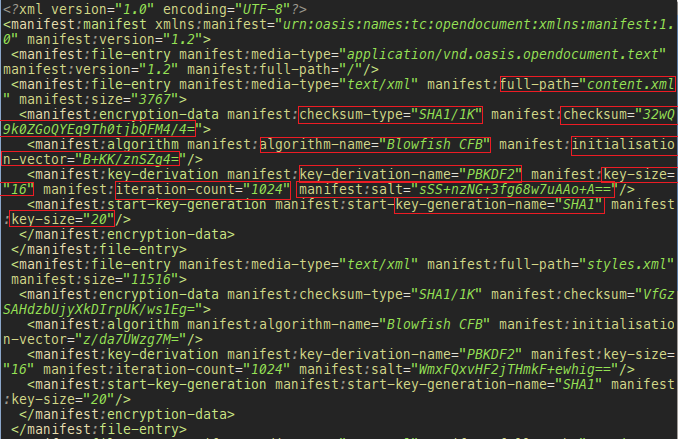
\includegraphics[scale=0.65]{resources/odf-manifest-final}
\end{figure}


Benchmarks, 

\shadowbox{\begin{minipage}[t]{1\textwidth}%
\renewcommand{\lstlistingname}{Code}
\lstset{tabsize=2,breaklines=true,numbers=left,basicstyle=\footnotesize\ttfamily,xleftmargin=30pt}
\lstinputlisting[language=bash,title=ODF cracking benchmarks]{resources/odf_output.txt}
\vspace{0.2cm}%
\end{minipage}}

http://cpan.uwinnipeg.ca/htdocs/Spreadsheet-ParseExcel/Spreadsheet/ParseExcel.pm.html\#Decryption

http://www.password-crackers.com/blog/?p=16

http://www.password-crackers.com/en/articles/12/\#II


\subsection{Guaranteed decryption of Office files using 40-bit RC4 encryption}

The Open Document Format for Office Applications (ODF), also known
as OpenDocument (OD), is an XML-based file format for spreadsheets,
charts, presentations and word processing documents. Our work is the
first open-source multi-core cracking software for ODF files. Uses
PBKDF2. OpenDocument files can also take the format of a ZIP compressed
archive containing a number of files and directories; these can contain
binary content and benefit from ZIP's lossless compression to reduce
Benchmarks, 

\shadowbox{\begin{minipage}[t]{1\textwidth}%
\renewcommand{\lstlistingname}{Code}
\lstset{tabsize=2,breaklines=true,numbers=left,basicstyle=\footnotesize\ttfamily,xleftmargin=30pt}
\lstinputlisting[language=bash,title=ODF cracking benchmarks]{resources/odf_output.txt}
\vspace{0.2cm}%
\end{minipage}}


\subsection{Office 2003 file encryption}


\subsection{Office 2007 file encryption}

The Open Document Format for Office Applications (ODF), also known
as OpenDocument (OD), is an XML-based file format for spreadsheets,
charts, presentations and word processing documents. Our work is the
first open-source multi-core cracking software for ODF files. Uses
PBKDF2. OpenDocument files can also take the format of a ZIP compressed
archive containing a number of files and directories; these can contain
binary content and benefit from ZIP's lossless compression to reduce.

\begin{figure}[H]
\caption{manifest.xml snipped sample}


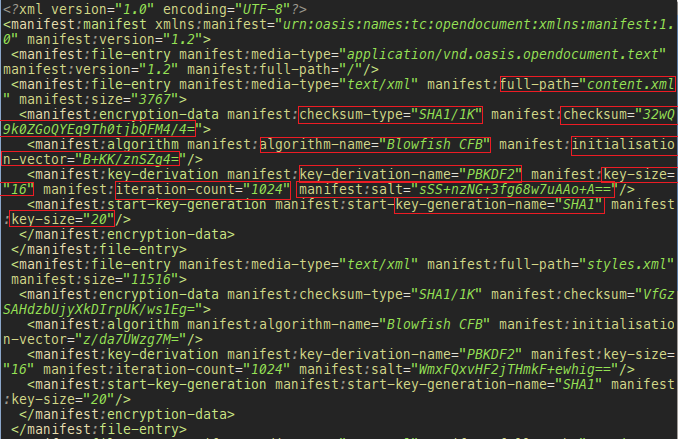
\includegraphics[scale=0.65]{resources/odf-manifest-final}
\end{figure}


Benchmarks, 

\shadowbox{\begin{minipage}[t]{1\textwidth}%
\renewcommand{\lstlistingname}{Code}
\lstset{tabsize=2,breaklines=true,numbers=left,basicstyle=\footnotesize\ttfamily,xleftmargin=30pt}
\lstinputlisting[language=bash,title=ODF cracking benchmarks]{resources/odf_output.txt}
\vspace{0.2cm}%
\end{minipage}}


\subsection{Office 2010 file encryption}

The Open Document Format for Office Applications (ODF), also known
as OpenDocument (OD), is an XML-based file format for spreadsheets,
charts, presentations and word processing documents. Our work is the
first open-source multi-core cracking software for ODF files. Uses
PBKDF2. OpenDocument files can also take the format of a ZIP compressed
archive containing a number of files and directories; these can contain
binary content and benefit from ZIP's lossless compression to reduce.

\begin{figure}[H]
\caption{manifest.xml snipped sample}


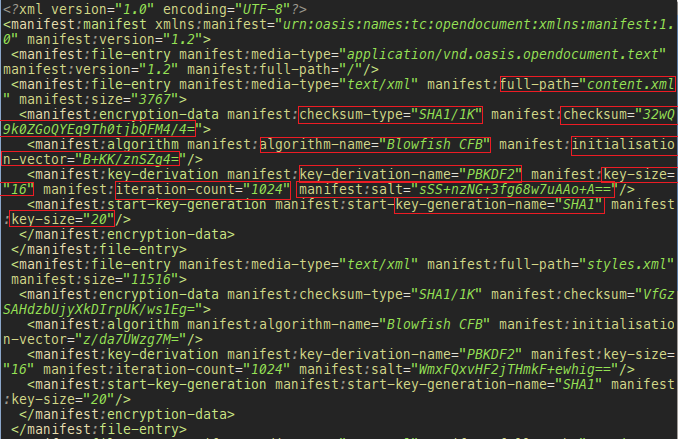
\includegraphics[scale=0.65]{resources/odf-manifest-final}
\end{figure}


Benchmarks, 

\shadowbox{\begin{minipage}[t]{1\textwidth}%
\renewcommand{\lstlistingname}{Code}
\lstset{tabsize=2,breaklines=true,numbers=left,basicstyle=\footnotesize\ttfamily,xleftmargin=30pt}
\lstinputlisting[language=bash,title=ODF cracking benchmarks]{resources/odf_output.txt}
\vspace{0.2cm}%
\end{minipage}}

Construct 2 file format tables from office2john.c.


\subsection{Office 2013 file encryption}

The Open Document Format for Office Applications (ODF), also known
as OpenDocument (OD), is an XML-based file format for spreadsheets,
charts, presentations and word processing documents. Our work is the
first open-source multi-core cracking software for ODF files. Uses
PBKDF2. OpenDocument files can also take the format of a ZIP compressed
archive containing a number of files and directories; these can contain
binary content and benefit from ZIP's lossless compression to reduce.

\begin{figure}[H]
\caption{manifest.xml snipped sample}


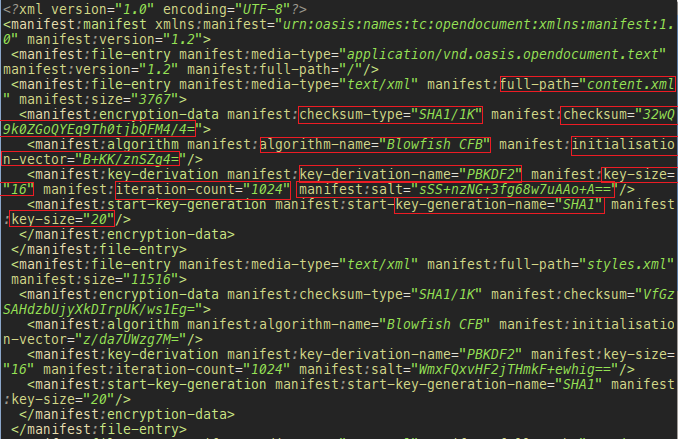
\includegraphics[scale=0.65]{resources/odf-manifest-final}
\end{figure}


Benchmarks, 

\shadowbox{\begin{minipage}[t]{1\textwidth}%
\renewcommand{\lstlistingname}{Code}
\lstset{tabsize=2,breaklines=true,numbers=left,basicstyle=\footnotesize\ttfamily,xleftmargin=30pt}
\lstinputlisting[language=bash,title=ODF cracking benchmarks]{resources/odf_output.txt}
\vspace{0.2cm}%
\end{minipage}}


\section{Analysis of OpenOffice / LibreOffice file format }

The Open Document Format for Office Applications (ODF), also known
as OpenDocument (OD), is an XML-based file format for spreadsheets,
charts, presentations and word processing documents. Our work is the
first open-source multi-core cracking software for ODF files. Uses
PBKDF2. OpenDocument files can also take the format of a ZIP compressed
archive containing a number of files and directories; these can contain
binary content and benefit from ZIP's lossless compression to reduce.

\begin{figure}[H]
\caption{manifest.xml snipped sample}


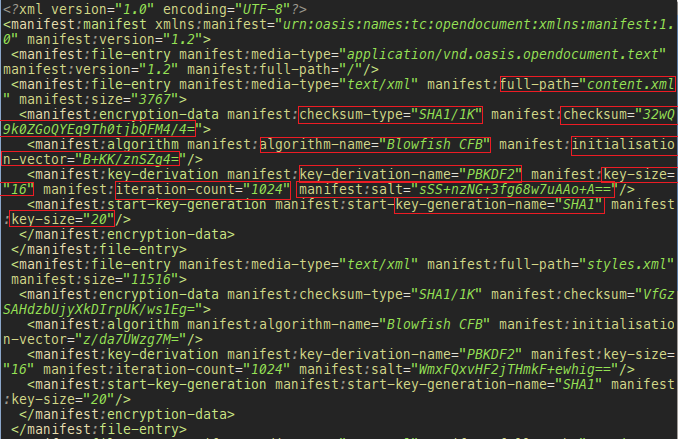
\includegraphics[scale=0.65]{resources/odf-manifest-final}
\end{figure}


Benchmarks, 

We compare the performance of ODF JtR plug-in on different machines
below,

\begin{figure}[H]
\caption{ODFcracking benchmarks}


\includegraphics[scale=0.75]{\string"resources/Agile Keychain Benchmarks\string".png}
\end{figure}


\shadowbox{\begin{minipage}[t]{1\textwidth}%
\renewcommand{\lstlistingname}{Code}
\lstset{tabsize=2,breaklines=true,numbers=left,basicstyle=\footnotesize\ttfamily,xleftmargin=30pt}
\lstinputlisting[language=bash,title=ODF cracking benchmarks]{resources/odf_output.txt}
\vspace{0.2cm}%
\end{minipage}}

By using techniques described in this section, it is possible to write
a cracker for earlier version of ODF files. See run/sxc2john.py and
src/sxc\_fmt\_plug.c file in JtR source tree.


\section{Analysis of PDF files }


\subsection{Analysis of PDF files using RC4 encryption}

\shadowbox{\begin{minipage}[t]{1\columnwidth}%
\renewcommand{\lstlistingname}{Code}
\lstset{tabsize=2,basicstyle=\ttfamily,breaklines=true,numbers=left,columns=flexible,xleftmargin=30pt}
\lstinputlisting[language=C,caption=PDF RC4 Cracker]{resources/pdf_rc4_cracker.c}
\vspace{0.2cm}%
\end{minipage}}


\subsection{Guaranteed decryption of PDF files using 40-bit RC4 encryption}

\shadowbox{\begin{minipage}[t]{1\columnwidth}%
\renewcommand{\lstlistingname}{Code}
\lstset{tabsize=2,basicstyle=\ttfamily,breaklines=true,numbers=left,columns=flexible,xleftmargin=30pt}
\lstinputlisting[language=C,caption=PDF 40-bit RC4 Cracker]{resources/pdf_sureshot_cracker.c}
\vspace{0.2cm}%
\end{minipage}}


\subsection{Adobe Acrobat 9 encrypted files (R5 algorithm)}

\shadowbox{\begin{minipage}[t]{1\columnwidth}%
\renewcommand{\lstlistingname}{Code}
\lstset{tabsize=2,basicstyle=\ttfamily,breaklines=true,numbers=left,columns=flexible,xleftmargin=30pt}
\lstinputlisting[language=C,caption=PDF 40-bit RC4 Cracker]{resources/pdf_sureshot_cracker.c}
\vspace{0.2cm}%
\end{minipage}}


\subsection{Analysis of Adobe Acrobat 10 and 11 encrypted files (R6 algorithm)}

\shadowbox{\begin{minipage}[t]{1\columnwidth}%
\renewcommand{\lstlistingname}{Code}
\lstset{tabsize=2,basicstyle=\ttfamily,breaklines=true,numbers=left,columns=flexible,xleftmargin=30pt}
\lstinputlisting[language=C,caption=PDF 40-bit RC4 Cracker]{resources/pdf_sureshot_cracker.c}
\vspace{0.2cm}%
\end{minipage}}


\subsection{Comparison of various KDF functions used in Adobe Acrobat}

We compare the performance of ODF JtR plug-in on different machines
below,

\begin{figure}[H]
\caption{ODFcracking benchmarks}


\includegraphics[scale=0.75]{\string"resources/Agile Keychain Benchmarks\string".png}
\end{figure}



\section{RAR files. }

RAR stands for Roshal ARchive and it is a proprietary archive file
format that supports data compression, error recovery, and file spanning.
RAR is a highly popular compression format embraced even by the software
cracking scene. The RAR file format is well documented in technote.txt. 

\begin{table}[H]
\caption{RAR file format}


\begin{tabular}{|>{\raggedright}m{2.5cm}|>{\raggedright}m{2.5cm}|>{\raggedright}m{6cm}|}
\hline 
Magic & 6 bytes & 0x9AA2D903, Magic\tabularnewline
\hline 
Version & 2 bytes & 0xB54BFB67, Magic\tabularnewline
\hline 
Cipher Name & 32 bytes & Determine what algorithms are used \tabularnewline
\hline 
Cipher Mode & 32 bytes & Version of the database format \tabularnewline
\hline 
Hash Spec & 32 bytes & Initial random number to start on the sha256 of the key \tabularnewline
\hline 
Payload Offset & 4 bytes & Initialization vector used for all algorithms \tabularnewline
\hline 
Key Bytes & 4 bytes & Encrypted 128 random value using P’ with Twofish algorithm\tabularnewline
\hline 
mkDigest  & 20 bytes & SHA1\tabularnewline
\hline 
mkDigestSalt & 32 bytes  & SHA256 hash of only the contents (entire file minus starting 124 bytes)\tabularnewline
\hline 
mkDigestIterations & 4 bytes  & Number of iterations in Phttp://en.wikipedia.org/wiki/Personal\_Storage\_TableBKDF2
function\tabularnewline
\hline 
UUID  & 40 & Number of rounds to do AES block encryption on the Master Key \tabularnewline
\hline 
keyblock structure (8 entries) & 48 bytes each & \tabularnewline
\hline 
\end{tabular}

Where, keyblock structure has the following format,

\begin{tabular}{|c|c|c|}
\hline 
active & 4 bytes & denotes whether this key slot is active or not\tabularnewline
\hline 
\hline 
passwordIterations & 4 bytes & parameters used for password processing\tabularnewline
\hline 
passwordSalt & 32 bytes & parameters used for password processing\tabularnewline
\hline 
keyMaterialOffset & 4 bytes & parameters used for AF store/load\tabularnewline
\hline 
stripes & 4 bytes & parameters used for AF store/load\tabularnewline
\hline 
\end{tabular}
\end{table}


RAR can encrypt data in two different way: First, in \textquotedbl{}-hp\textquotedbl{}
mode, both file data and file headers (which contains file names and
other metadata) are encrypted. Encryption algorithm is changed to
cipher block chaining (CBC) mode over AES (Advanced Encryption Standard)
with 128 bit key length.Encryption of both file data and file headers.
RAR uses custom key stretching algorithm to deter brute-force attacks.
In \textquotedbl{}-p\textquotedbl{} mode only file data is encrypted.
At first, it seems files encrypted using \textquotedbl{}-hp\textquotedbl{}
seem to offer more security since even the file headers are encrypted.
However, in practice file encrypted using -\textquotedbl{}hp\textquotedbl{}
can be attacked in two different way, 1) known partial plain-text
attack 2) File header CRC verification. File encrypted using \textquotedbl{}-p\textquotedbl{}
are harder to brute-force, the decrypted (but still compressed) file
data streams contain no information if they are valid compressed data
stream. Hence to attack \textquotedbl{}-p\textquotedbl{} mode files,
a full Un-RAR engine must be implemented which de-compresses the decrypted
data, the computes the CRC over un-compressed data and compares the
CRC with the value stored in the file header.

The \textquotedbl{}known partial plain-text attack\textquotedbl{}
on \textquotedbl{}-hp\textquotedbl{} mode files was first found out
Marc Bevland and used in his unrarhp tool. Our initiial implementation
of RAR cracker could only deal with \textquotedbl{}-hp\textquotedbl{}
mode files. It has been later extended by magnum (JtR jumbo's maintainer)
to support \textquotedbl{}-p\textquotedbl{} mode files. magnum has
even implemented GPU cracking support of RAR files!

{[}Insert RAR key stretching algorithm{]} {[}Insert RAR cracking snippet
for \textquotedbl{}-hp\textquotedbl{} mode RAR files{]} {[} Benchmark
CPU, our GPU, igrargpu{]}


\section{LUKS }

Linux Unified Key Setup or LUKS is a disk-encryption specification.
The reference implementation for LUKS operates on Linux and is based
on an enhanced version of cryptsetup, using dm-crypt as the disk encryption
backend. Device-mapper crypt (dm-crypt) target provides transparent
encryption of block devices using the kernel crypto API. LUKS is the
standard for Linux hard disk encryption. By providing a standard on-disk-format,
it does not only facilitate compatibility among distributions, but
also provides secure management of multiple user passwords. In contrast
to existing solution, LUKS stores all setup necessary setup information
in the partition header, enabling the user to transport or migrate
his data seamlessly. While LUKS is a standard on-disk format, there
is also a reference implementation. LUKS for dm-crypt is implemented
in an enhanced version of cryptsetup. cryptsetup is used to conveniently
setup dm-crypt managed block devices under Linux.

\begin{table}[H]
\caption{LUKS header fields (size is 208 bytes + 48 {*} LUKS\_NUMKEYS = 592
bytes)}


\begin{tabular}{|>{\raggedright}m{2.5cm}|>{\raggedright}m{2.5cm}|>{\raggedright}m{6cm}|}
\hline 
Magic & 6 bytes & 0x9AA2D903, Magic\tabularnewline
\hline 
Version & 2 bytes & 0xB54BFB67, Magic\tabularnewline
\hline 
Cipher Name & 32 bytes & Determine what algorithms are used \tabularnewline
\hline 
Cipher Mode & 32 bytes & Version of the database format \tabularnewline
\hline 
Hash Spec & 32 bytes & Initial random number to start on the sha256 of the key \tabularnewline
\hline 
Payload Offset & 4 bytes & Initialization vector used for all algorithms \tabularnewline
\hline 
Key Bytes & 4 bytes & Encrypted 128 random value using P’ with Twofish algorithm\tabularnewline
\hline 
mkDigest  & 20 bytes & SHA1\tabularnewline
\hline 
mkDigestSalt & 32 bytes  & SHA256 hash of only the contents (entire file minus starting 124 bytes)\tabularnewline
\hline 
mkDigestIterations & 4 bytes  & Number of iterations in PBKDF2 function\tabularnewline
\hline 
UUID  & 40 & Number of rounds to do AES block encryption on the Master Key \tabularnewline
\hline 
keyblock structure (8 entries) & 48 bytes each & \tabularnewline
\hline 
\end{tabular}

Where, keyblock structure has the following format,

\begin{tabular}{|c|c|c|}
\hline 
active & 4 bytes & denotes whether this key slot is active or not\tabularnewline
\hline 
\hline 
passwordIterations & 4 bytes & parameters used for password processing\tabularnewline
\hline 
passwordSalt & 32 bytes & parameters used for password processing\tabularnewline
\hline 
keyMaterialOffset & 4 bytes & parameters used for AF store/load\tabularnewline
\hline 
stripes & 4 bytes & parameters used for AF store/load\tabularnewline
\hline 
\end{tabular}
\end{table}


Our naive brute-force software (based on Revelation Python sources)
is super slow and achieves a speed of merely 0.3 p/s. This slowness
can be partially attributed to interpretive nature of Python code.
Our second implementation in C (based on official cryptsetup sources)
is three times faster and achieves roughly 1 p/s. {[}Give estimates
for cracking 8 byte alpha and alphanumeric passwords{]}. LUKS has
upto 8 key slots. One clever attack is that we can choose to attack
a key slot which has minimum cryptographic strength (i.e use lesser
iterations in its key derivation function). Can I use LUKS or cryptsetup
with a more secure (external) medium for key storage, e.g. TPM or
a smartcard? Yes, see the answers on using a file-supplied key. You
do have to write the glue-logic yourself though. Basically you can
have cryptsetup read the key from STDIN and write it there with your
own tool that in turn gets the key from the more secure key storage. 


\section{Analysis of TrueCrypt }

TrueCrypt \citep{TCF:2004} is a popular on-the-fly encryption. It
can create a file-hosted container or write a partition which consists
of an encrypted volume with its own file system (contained within
a regular file) which can then be mounted as if it were a real disk.
TrueCrypt also supports device-hosted volumes, which can be created
on either an individual partition or an entire disk. Because presence
of a TrueCrypt volume can not be verified without the password, disk
and filesystems utilities may report the filesystem as unformatted
or corrupted that may lead to data loss after incorrect user intervention
or automatic \textquotedbl{}repair\textquotedbl{}. 

The standard volume header uses the first 512 bytes of the TrueCrypt
container. It contains the master keys needed to decrypt the volume.
The 512 bytes hidden volume header is stored 1536 bytes from the end
of the host volume. TrueCrypt volumes have no \textquotedbl{}signature\textquotedbl{}
or ID strings. Until decrypted, they appear to consist solely of random
data. 

Free space on each TrueCrypt volume is filled with random data when
the volume is created.

It is not possible to identify TrueCrypt containers by simply looking
for some well-defined magic string. This provides strong deniability.
Information about the exact PKBDF2 function and cipher(s) used in
an encrypted container is not stored in the header. As a consequence
all possible combination must be tried. This slow down the brute force
attack considerably. The various possible PBKDF2 algorithms used by
TrueCrypt are : PBKDF2-HMAC-SHA256 with 2000 rounds etc. The various
possible encrytion ciphers (including chained ciphers) are AES-XTS
etc.

\begin{table}[H]
\caption{TrueCrypt Volume Format Specification (512 bytes)}
\vspace{0.3cm}

\begin{tabular}{|>{\raggedright}m{2cm}|>{\raggedright}m{1.5cm}|>{\raggedright}m{2cm}|>{\raggedright}m{6cm}|}
\hline 
SALT & 64 & Unencrypted & Salt\tabularnewline
\hline 
MAGIC & 4 bytes & Encrypted & ASCII string \textquotedbl{}TRUE\textquotedbl{}\tabularnewline
\hline 
Version & 2 bytes & Encrypted & Volume header format version\tabularnewline
\hline 
Min. Version & 2 bytes & Encrypted & Encrypted\tabularnewline
\hline 
crc\_keys & 4 bytes & Encrypted & CRC32 of the key section\tabularnewline
\hline 
vol\_ctime & 8 bytes & Encrypted & Volume creation time\tabularnewline
\hline 
hdr\_ctime & 8 bytes & Encrypted & Header creation time\tabularnewline
\hline 
sz\_hidvol & 8 bytes & Encrypted & Size of hidden volume\tabularnewline
\hline 
sz\_vol & 8 bytes & Encrypted & Size of volume\tabularnewline
\hline 
off\_mk\_scope & 8 bytes & Encrypted & Byte offset of the start of the master key scope\tabularnewline
\hline 
sz\_mk\_scope & 8 bytes & Encrypted & Size of the encrypted area withint he master key scope\tabularnewline
\hline 
Flags & 4 bytes & Encrypted & Flag bits\tabularnewline
\hline 
sec\_sz & 4 bytes & Encrypted & Sector size (in bytes)\tabularnewline
\hline 
unused & 120 bytes & Encrypted & Reserved\tabularnewline
\hline 
crc\_dhdr & 4 bytes & Encrypted & CRC32 of decrypted header (except keys)\tabularnewline
\hline 
keys & 256 bytes & Encrypted & Concatenated primary and secondary master keys\tabularnewline
\hline 
\end{tabular}
\end{table}


Benchmarks of all TC crackers out there (Excel bar chart). 

\shadowbox{\begin{minipage}[t]{1\textwidth}%
\renewcommand{\lstlistingname}{Code}
\lstset{tabsize=2,breaklines=true,numbers=left,basicstyle=\footnotesize\ttfamily,xleftmargin=30pt}
\lstinputlisting[language=bash,title=Pseudo-code for cracking TrueCrypt volume]{resources/django_output.txt}
\vspace{0.2cm}%
\end{minipage}}

Also mention real-life usage of these tools in competition ;)

\shadowbox{\begin{minipage}[t]{1\textwidth}%
\renewcommand{\lstlistingname}{Code}
\lstset{tabsize=2,breaklines=true,numbers=left,basicstyle=\footnotesize\ttfamily,xleftmargin=30pt}
\lstinputlisting[language=C,title=VNC cracking ]{resources/vnc_algorithm.c}
\vspace{0.2cm}%
\end{minipage}}


\section{.pfx / .p12 files }

Work in progress.

JtR-jumbo is a community enhanced version of JtR with 

{[}Compiled debug version of OpenSSL to trace which encryption functions
are called{]}

Compare our \textquotedbl{}trivial\textquotedbl{} cracker with Elcomsoft's
EDPR (get benchmarks from all servers).

It defines a file format commonly used to store X.509 private keys
with accompanying public key certificates, protected with a password-based
symmetric key, and is the successor to PFX from Microsoft. PFX has
received heavy criticism of being one of the most complex cryptographic
protocols,{[}1{]} but nevertheless remains the only standard way today
to store private keys and certificates in a single encrypted file.

Our .P12 cracker cheats by not not implementing its own crypto functions,
instead it replies on OpenSSL's verifyxyz function to do the heavy
lifting.

http://www.drh-consultancy.demon.co.uk/pkcs12faq.html/

\#12 supports the following encryption algorithms.

128 bit RC4 with SHA1 40 bit RC4 with SHA1 3 key triple DES with SHA1
(168 bits) 2 key triple DES with SHA1 (112 bits) 128 bit RC2 with
SHA1 40 bit RC2 with SHA1

In addition the PKCS\#5 v1.5 modes are possible as well. This also
permits the following.

DES with MD5 (56bit) DES with MD2 (56bit)

What's this I hear about iteration counts? A. The algorithm used to
generate keys from passwords and the MAC has an optional iteration
count. This determines how many times part of the algorithm is repeated.
It's a way of slowing down the key derivation process to make it harder
to make dictionary attacks on the password. The -info option now prints
information about iteration counts. Q. What iteration counts are used?

A. By default I set both iteration counts to 2048. If you use the
-nomaciter option the MAC iteration count is also set to 1 some software
such as MSIE4 needs this option because it does not support mac iteration
counts. If you use the noiter option the iteration count is set to
1: since this makes dictionary attacks on the password easier this
is not recommended.

MSIE5 uses 2000 for the encryption iteration count. If you have the
'enable strong protection' option checked then it uses 2000 for the
MAC count otherwise it uses 1 (for compatability with earlier versions
of MSIE).

ftp://ftp.rsasecurity.com/pub/pkcs/pkcs-12/pkcs-12v1.pdf

Both are PKCS \#12 files (Personal Information Exchange Syntax)


\section{Mozilla master passwords }

implements the only multi-core open-source RACF hash cracking software.

\shadowbox{\begin{minipage}[t]{1\textwidth}%
\renewcommand{\lstlistingname}{Code}
\lstset{tabsize=2,breaklines=true,numbers=left,basicstyle=\footnotesize\ttfamily,xleftmargin=30pt}
\lstinputlisting[language=Python,caption=RACF hashing algorithm]{resources/racf_algorithm.py}
\vspace{0.2cm}%
\end{minipage}}

Research into the RACF system was done in collaboration with Nigel
Pentland (author of CRACF) and Phil Young. 

\shadowbox{\begin{minipage}[t]{1\columnwidth}%
\renewcommand{\lstlistingname}{Code}
\lstset{tabsize=2,breaklines=true,numbers=left,basicstyle=\footnotesize\ttfamily,xleftmargin=30pt}
\lstinputlisting[language=bash,title=RACF cracker benchmarks]{resources/racf_output.txt}
\vspace{0.2cm}%
\end{minipage}}


\section{Analysis of encrypted 7-Zip files }

Work in progress.


\chapter{Analysis of security of various authentication protocols \label{chap:auth-protocols}}


\section{Kerberos v5 authentication protocol }

Kerberos is a computer network authentication protocol which works
on the basis of \textquotedbl{}tickets\textquotedbl{} to allow nodes
communicating over a non-secure network to prove their identity to
one another in a secure manner .

\shadowbox{\begin{minipage}[t]{1\textwidth}%
\renewcommand{\lstlistingname}{Code}
\lstset{tabsize=2,breaklines=true,numbers=left,basicstyle=\footnotesize\ttfamily,xleftmargin=25pt}
\lstinputlisting[language=C,caption=LastPass Cracker]{resources/lastpass_algorithm.c}
\vspace{0.2cm}%
\end{minipage}}

Essentially we decrypt the encrypted\_username value and compare it
against the original username to verify if the gived password was
correct or not. For details see src/lastpass\_fmt\_plug.c in JtR source
tree. 

We compare the performance of LastPass cracker on different machines
below,

\begin{figure}[H]
\caption{LastPass Cracking Benchmarks}


\includegraphics[scale=0.75]{\string"resources/Agile Keychain Benchmarks\string".png}
\end{figure}


\shadowbox{\begin{minipage}[t]{1\columnwidth}%
\renewcommand{\lstlistingname}{Benchmarks} 
\lstset{tabsize=2,basicstyle=\footnotesize\ttfamily,breaklines=true,xleftmargin=30pt}
\lstinputlisting[language=bash,title=LastPass cracking benchmarks]{resources/kwallet_output.txt}
\vspace{0.2cm}
%
\end{minipage}}

Describe Ettercap + JtR work


\section{MongoDB authentication protocol }

DONE. At least it has some protection unlike Redis which sends the
password in clear text

\shadowbox{\begin{minipage}[t]{1\textwidth}%
\renewcommand{\lstlistingname}{Code}
\lstset{tabsize=2,breaklines=true,numbers=left,basicstyle=\footnotesize\ttfamily,xleftmargin=25pt}
\lstinputlisting[language=C,caption=LastPass Cracker]{resources/lastpass_algorithm.c}
\vspace{0.2cm}%
\end{minipage}}

Essentially we decrypt the encrypted\_username value and compare it
against the original username to verify if the gived password was
correct or not. For details see src/lastpass\_fmt\_plug.c in JtR source
tree. 

We compare the performance of LastPass cracker on different machines
below,

\begin{figure}[H]
\caption{LastPass Cracking Benchmarks}


\includegraphics[scale=0.75]{\string"resources/Agile Keychain Benchmarks\string".png}
\end{figure}


\shadowbox{\begin{minipage}[t]{1\columnwidth}%
\renewcommand{\lstlistingname}{Benchmarks} 
\lstset{tabsize=2,basicstyle=\footnotesize\ttfamily,breaklines=true,xleftmargin=30pt}
\lstinputlisting[language=bash,title=LastPass cracking benchmarks]{resources/kwallet_output.txt}
\vspace{0.2cm}
%
\end{minipage}}

Describe Ettercap + JtR work


\section{MySQL challenge-response authentication protocol }

DONE. Describe Ettercap + JtR work

\shadowbox{\begin{minipage}[t]{1\textwidth}%
\renewcommand{\lstlistingname}{Code}
\lstset{tabsize=2,breaklines=true,numbers=left,basicstyle=\footnotesize\ttfamily,xleftmargin=25pt}
\lstinputlisting[language=C,caption=LastPass Cracker]{resources/lastpass_algorithm.c}
\vspace{0.2cm}%
\end{minipage}}

Essentially we decrypt the encrypted\_username value and compare it
against the original username to verify if the gived password was
correct or not. For details see src/lastpass\_fmt\_plug.c in JtR source
tree. 

We compare the performance of LastPass cracker on different machines
below,

\begin{figure}[H]
\caption{LastPass Cracking Benchmarks}


\includegraphics[scale=0.75]{\string"resources/Agile Keychain Benchmarks\string".png}
\end{figure}


\shadowbox{\begin{minipage}[t]{1\columnwidth}%
\renewcommand{\lstlistingname}{Benchmarks} 
\lstset{tabsize=2,basicstyle=\footnotesize\ttfamily,breaklines=true,xleftmargin=30pt}
\lstinputlisting[language=bash,title=LastPass cracking benchmarks]{resources/kwallet_output.txt}
\vspace{0.2cm}
%
\end{minipage}}

Describe Ettercap + JtR work


\section{PostgreSQL authentication protocol }

DONE. Describe Ettercap + JtR + Nmap + Metasploit work. Man in the
middle downgrade attack.

\shadowbox{\begin{minipage}[t]{1\textwidth}%
\renewcommand{\lstlistingname}{Code}
\lstset{tabsize=2,breaklines=true,numbers=left,basicstyle=\footnotesize\ttfamily,xleftmargin=25pt}
\lstinputlisting[language=C,caption=LastPass Cracker]{resources/lastpass_algorithm.c}
\vspace{0.2cm}%
\end{minipage}}

Essentially we decrypt the encrypted\_username value and compare it
against the original username to verify if the gived password was
correct or not. For details see src/lastpass\_fmt\_plug.c in JtR source
tree. 

We compare the performance of LastPass cracker on different machines
below,

\begin{figure}[H]
\caption{LastPass Cracking Benchmarks}


\includegraphics[scale=0.75]{\string"resources/Agile Keychain Benchmarks\string".png}
\end{figure}


\shadowbox{\begin{minipage}[t]{1\columnwidth}%
\renewcommand{\lstlistingname}{Benchmarks} 
\lstset{tabsize=2,basicstyle=\footnotesize\ttfamily,breaklines=true,xleftmargin=30pt}
\lstinputlisting[language=bash,title=LastPass cracking benchmarks]{resources/kwallet_output.txt}
\vspace{0.2cm}
%
\end{minipage}}

Describe Ettercap + JtR work


\section{Oracle O5LOGON protocol }

DONE. Describe Ettercap + JtR + Nmap work

\shadowbox{\begin{minipage}[t]{1\textwidth}%
\renewcommand{\lstlistingname}{Code}
\lstset{tabsize=2,breaklines=true,numbers=left,basicstyle=\footnotesize\ttfamily,xleftmargin=25pt}
\lstinputlisting[language=C,caption=LastPass Cracker]{resources/lastpass_algorithm.c}
\vspace{0.2cm}%
\end{minipage}}

Essentially we decrypt the encrypted\_username value and compare it
against the original username to verify if the gived password was
correct or not. For details see src/lastpass\_fmt\_plug.c in JtR source
tree. 

We compare the performance of LastPass cracker on different machines
below,

\begin{figure}[H]
\caption{LastPass Cracking Benchmarks}


\includegraphics[scale=0.75]{\string"resources/Agile Keychain Benchmarks\string".png}
\end{figure}


\shadowbox{\begin{minipage}[t]{1\columnwidth}%
\renewcommand{\lstlistingname}{Benchmarks} 
\lstset{tabsize=2,basicstyle=\footnotesize\ttfamily,breaklines=true,xleftmargin=30pt}
\lstinputlisting[language=bash,title=LastPass cracking benchmarks]{resources/kwallet_output.txt}
\vspace{0.2cm}
%
\end{minipage}}

Describe Ettercap + JtR work


\section{iSCSI CHAP authentication protocol }

iSCSI (Internet Small Computer System Interface) is an Internet Protocol
(IP) based networking standard for linking storage facilities. iSCSI
allows clients (called initiators) to send SCSI commands (CDBs) to
SCSI storage devices (targets) on remote servers to facililate data
transfer. It is a storage area network (SAN) protocol, allowing organizations
to consolidate storage into data center storage arrays while providing
hosts (such as database and web servers) with the illusion of locally
attached disks.

iSCSI targets can be password protected by using CHAP protocol. <Decribe
algorithm>.We have extended Ettercap to sniff and decode the key packets
involved in iSCSI CHAP authentication protocol.

\begin{figure}[H]
\caption{iSCSI initiator to target packet}


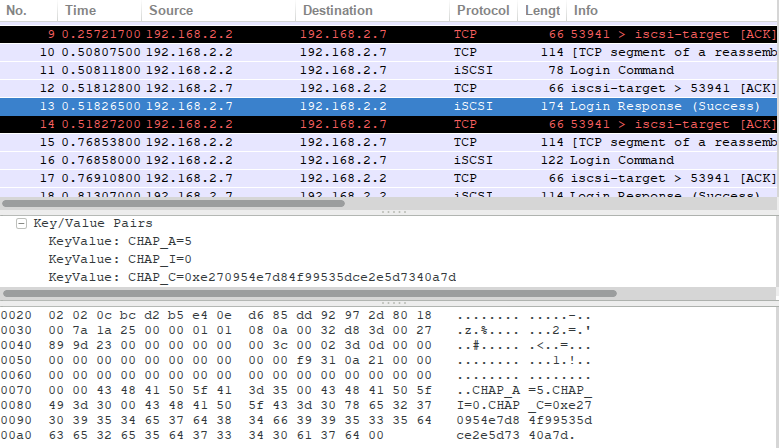
\includegraphics[scale=0.4]{resources/iSCSI-1}
\end{figure}


\begin{figure}[H]
\caption{iSCSI target to initiator packet}


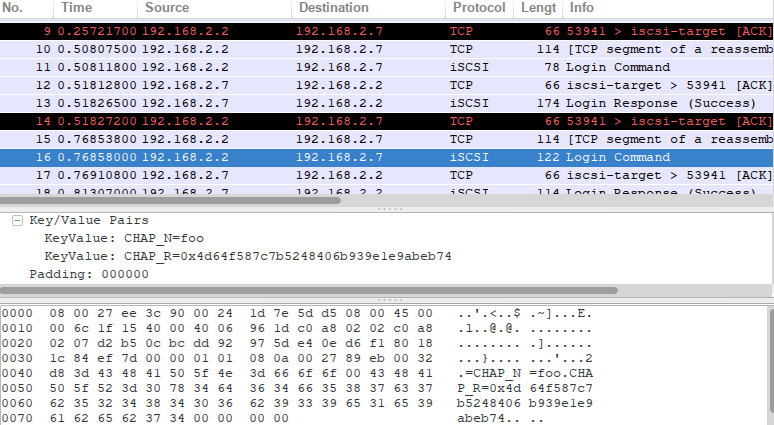
\includegraphics[scale=0.4]{resources/iSCSI-2}
\end{figure}


We have written a custom cracker for sniffed iSCSI CHAP authentication
hashes and the following snippet shows the main steps involved,

\shadowbox{\begin{minipage}[t]{1\textwidth}%
\renewcommand{\lstlistingname}{Code}
\lstset{tabsize=2,breaklines=true,numbers=left,basicstyle=\footnotesize\ttfamily,xleftmargin=25pt}
\lstinputlisting[language=C,caption=iSCSI Cracker]{resources/lastpass_algorithm.c}
\vspace{0.2cm}%
\end{minipage}}

Essentially we decrypt the encrypted\_username value and compare it
against the original username to verify if the gived password was
correct or not. For details see src/lastpass\_fmt\_plug.c in JtR source
tree. 

We compare the performance of LastPass cracker on different machines
below,

\begin{figure}[H]
\caption{iSCSI Cracking Benchmarks}


\includegraphics[scale=0.75]{\string"resources/Agile Keychain Benchmarks\string".png}
\end{figure}


\shadowbox{\begin{minipage}[t]{1\columnwidth}%
\renewcommand{\lstlistingname}{Benchmarks} 
\lstset{tabsize=2,basicstyle=\footnotesize\ttfamily,breaklines=true,xleftmargin=30pt}
\lstinputlisting[language=bash,title=iSCSI cracking benchmarks]{resources/kwallet_output.txt}
\vspace{0.2cm}
%
\end{minipage}}

Describe Ettercap + JtR work


\section{VNC protocol }

Virtual Network Computing (VNC) is a graphical desktop sharing system
that uses the RFB protocol (remote framebuffer) to remotely control
another computer. It transmits the keyboard and mouse events from
one computer to another, relaying the graphical screen updates back
in the other direction, over a network. VNC is platform-independent
– a VNC viewer on one operating system may connect to a VNC server
on the same or any other operating system. A VNC system consists of
a client, a server, and a communication protocol. The VNC server is
the program on the machine that shares its screen. The server passively
allows the client to take control of it. The VNC client (or viewer)
is the program that watches, controls, and interacts with the server.
The client controls the server. The VNC protocol (RFB) is very simple,
based on one graphic primitive from server to client (\textquotedbl{}Put
a rectangle of pixel data at the specified X,Y position\textquotedbl{})
and event messages from client to server. VNC by default uses TCP
port 5900+N,{[}5{]}{[}6{]} where N is the display number. The first
step in attacking VNC cracking involves passive sniffing of the VNC
traffic. Once the traffic has been captured.

VNC encryption key can be potentially broken only by mere passive
sniffing of the traffic. In our opinion, VNC authentication protocol
offers poor security and hasn't been fixed even in the newer versions
of the RFB protocol.

{[}Paste wireshark screenshots{]} 

\shadowbox{\begin{minipage}[t]{1\textwidth}%
\renewcommand{\lstlistingname}{Code}
\lstset{tabsize=2,breaklines=true,numbers=left,basicstyle=\footnotesize\ttfamily,xleftmargin=25pt}
\lstinputlisting[language=C,caption=LastPass Cracker]{resources/lastpass_algorithm.c}
\vspace{0.2cm}%
\end{minipage}}

Essentially we decrypt the encrypted\_username value and compare it
against the original username to verify if the gived password was
correct or not. For details see src/lastpass\_fmt\_plug.c in JtR source
tree. 

We compare the performance of LastPass cracker on different machines
below,

\begin{figure}[H]
\caption{LastPass Cracking Benchmarks}


\includegraphics[scale=0.75]{\string"resources/Agile Keychain Benchmarks\string".png}
\end{figure}


\shadowbox{\begin{minipage}[t]{1\columnwidth}%
\renewcommand{\lstlistingname}{Benchmarks} 
\lstset{tabsize=2,basicstyle=\footnotesize\ttfamily,breaklines=true,xleftmargin=30pt}
\lstinputlisting[language=bash,title=LastPass cracking benchmarks]{resources/kwallet_output.txt}
\vspace{0.2cm}
%
\end{minipage}}

Describe Ettercap + JtR work


\section{LastPass authentication protocol }

LastPass is a free online password manager and Form Filler that makes
your web browsing easier and more secure. User's sensitive data is
encrypted locally before upload so even LastPass cannot get access
to it \citet{LastPass}. LastPass Password Manager protects passwords
by using local AES encryption and a master password.

LastPass Password Manager is a closed source software and uses a proprietary
file format. Earlier versions of LastPass used a weak KDF function
and were susceptible to brute foce at high speeds (see \citet{LastPass + Belenko}).
However \citet{LastPass + Belenko} is secretive (being from a commercial
password cracking company) and does not contain any internal details.
The lastest verions of LastPass Password Manager employ PBKDF2-SHA256
with variable number of iterations to slow down brute-force attacks. 

In this work, we present security analysis of the lastest version
of LastPass Password Manager. LastPass denied our requests to open
up their proprietary file format for third-party security analysis.
So, instead of analyzing the LastPass file format and finding possible
offline attacks against it, we shifted to studying the authentication
protocol used by LastPass.

The following screenshot shows the traffic exchanged between the LastPass
Password Manager plug-in (running in the browser) and LastPass backend
servers,

\begin{figure}[H]
\caption{LastPass authentication protocol}


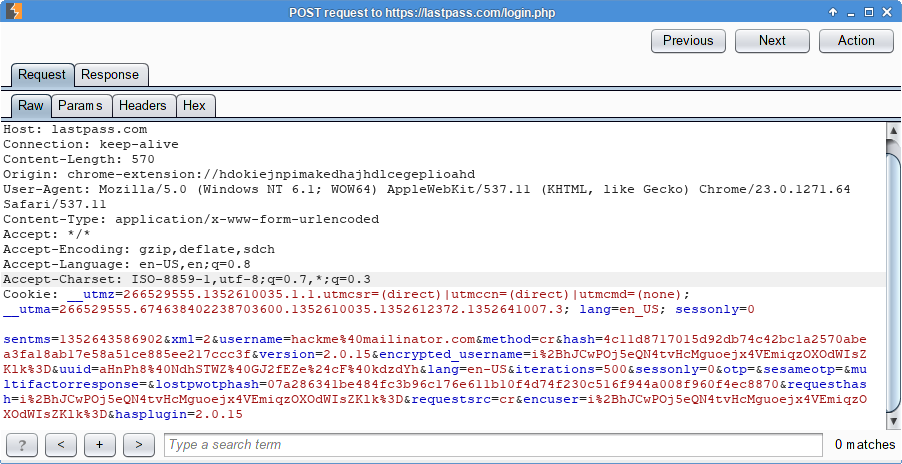
\includegraphics[scale=0.35]{resources/LastPass_sniff}
\end{figure}


After some analsysis, we found out that the query parameter ``encrypted\_username''
is essentially username (known value) encrypted with a key derived
from user password. LastPass uses a PBKDF2 as its key derivation function.
We have written a custom cracker for sniffed LastPass authentication
traffic and the following snippet shows the main steps involved,

\shadowbox{\begin{minipage}[t]{1\textwidth}%
\renewcommand{\lstlistingname}{Code}
\lstset{tabsize=2,breaklines=true,numbers=left,basicstyle=\footnotesize\ttfamily,xleftmargin=25pt}
\lstinputlisting[language=C,caption=LastPass Cracker]{resources/lastpass_algorithm.c}
\vspace{0.2cm}%
\end{minipage}}

Essentially we decrypt the encrypted\_username value and compare it
against the original username to verify if the gived password was
correct or not. For details see src/lastpass\_fmt\_plug.c in JtR source
tree. 

We compare the performance of LastPass cracker on different machines
below,

\begin{figure}[H]
\caption{LastPass Cracking Benchmarks}


\includegraphics[scale=0.75]{\string"resources/Agile Keychain Benchmarks\string".png}
\end{figure}


\shadowbox{\begin{minipage}[t]{1\columnwidth}%
\renewcommand{\lstlistingname}{Benchmarks} 
\lstset{tabsize=2,basicstyle=\footnotesize\ttfamily,breaklines=true,xleftmargin=30pt}
\lstinputlisting[language=bash,title=LastPass cracking benchmarks]{resources/kwallet_output.txt}
\vspace{0.2cm}
%
\end{minipage}}

Offline attacks on LastPass offline database are work in progress.


\section{Clipperz authentication protocol }

Clipperz is a popular free online password manager \citet{Clipperz}.
It does encryption on the local browser which gurantees confidentiality
of data. Clipperz supports exporting encrypted databases into offline
versions. Offline versions use the same cryptographic technology as
used by the online version.

Clipperz does not believe in ``security through obscurity'' (unlike
LastPass) and all the code behing Clipperz is open-source \citet{Clipperz github}.
Clipperz uses SRP (Secure Remote Password protocol, see \citet{SRP 1},
\citet{SRP 2} and \citet{SRP algorithm}) for online and offline
authentication. SRP is essentailly an authentication protocol for
password-based, mutual authentication over an insecure network connection
and requires both sides of the connection to have knowledge of the
user’s password. SRP offers security and deployment advantages over
other challenge-response protocols, such as Kerberos and SSL, in that
it does not require trusted key servers or certificate infrastructures.
Instead, small verification keys derived from each user’s password
are stored and used by each SRP server application \citet{SRP algorithm}.
``SRP does not store plaintext passwords on the server side but instead
uses what is known as a “non plaintext-equivalent verifier” \citet{Clipperz Details}.

Password verifier is derived from a Private key (called x) by using
the formula v = g\textasciicircum{}x, where x (Private key) = H(s,
H( I | ‘:’ | p )), g is generator modulo N, I is username, p is cleartext
password, H() is one-way hash function and s is salt. In theory, ``compromized
verification keys (called v) are of little value to an attacker''.
However in practice, it is possible to brute-force the original password
from the verification key at high speeds.

Ideally, for increassed resistance against brute-force attacks, a
costly (slow) one-way hash function (H) like PBKDF2 should be used.
However, in reality we have seen very fast hash functions (like single
iterations of SHA1 or SHA256) being used (See\citet{Clipperz} and
\citet{Blizzard SRP}). This allows an attacker to mount brute-force
attack at high-speeds.

The following snippet show how the salt and the verifier (verification
key) are stored in the database,

\shadowbox{\begin{minipage}[t]{1\textwidth}%
\renewcommand{\lstlistingname}{Code}
\lstset{tabsize=2,breaklines=true,numbers=none,basicstyle=\footnotesize\ttfamily,xleftmargin=30pt}
\lstinputlisting[language=bash,title=Clipperz secret data]{resources/clipperz_metadata.txt}
\vspace{0.2cm}%
\end{minipage}}

The following snippet shows how we can derive a verifer from a given
salt and user password and check if the gives user password was correct,

\shadowbox{\begin{minipage}[t]{1\textwidth}%
\renewcommand{\lstlistingname}{Code}
\lstset{tabsize=2,breaklines=true,numbers=none,basicstyle=\footnotesize\ttfamily,xleftmargin=30pt}
\lstinputlisting[language=Python,title=Clipperz Cracker]{resources/clipperz_algorithm.txt}
\vspace{0.2cm}%
\end{minipage}}

For details see src/clipperz\_fmt\_plug.c in JtR source tree. We compare
the performance of Clipperz cracker on different machines below,

\begin{figure}[H]
\caption{Clipperz Cracking Benchmarks}


\includegraphics[scale=0.75]{\string"resources/Agile Keychain Benchmarks\string".png}
\end{figure}


\shadowbox{\begin{minipage}[t]{1\columnwidth}%
\renewcommand{\lstlistingname}{Benchmarks} 
\lstset{tabsize=2,basicstyle=\footnotesize\ttfamily,breaklines=true,xleftmargin=30pt}
\lstinputlisting[language=bash,title=Clipperz cracking benchmarks]{resources/kwallet_output.txt}
\vspace{0.2cm}
%
\end{minipage}}


\chapter{Analysis of security of various backup solution. \label{chap:backup-solutions}}


\section{Analysis of Dropbox}


\section{Analysis of inSync Druva}

Druva inSync is an on-premise and cloud-based backup software. Druva
provides enterprise laptop backup solutions that protect corporate
users data with 10x faster backups and 90\% reduction in storage requirements.
The data encrypted both during transit (256-bit SSL) and in the storage
(256-bit AES) 1,576 enterprises. 


\subsubsection{1,126,840 endpoints, 46 countries, 98\% Customer Satisfaction Rate,
Customers include NASA, PwC, Deloitte, Amway and McAfee among others}

Rated “excellent” by Gartner. inSync Cloud offers the industry-best
security.

SAS 70 Type II, PCI DSS Level 1, ISO 27001, ISAE 3000 Type I

Industry-First Two-Factor Encryption. Even Druva can’t access your
data.

How do they de-deduplication? Does “dropship” like attack works?

“inSync Cloud offers the industry-best security”


\subsection{Authetication Issues}

Uses single iteration of md5 to protect admin and user passwords.
hash = md5(id + password)

select id, name, emailid, password from administrator

Such hashes are crackable at high speeds using JtR or hashcat family
of softwares. (4.2B c/s possible with oclHashcat-lite on AMD 7970)

Fix: use PBKDF2

“inSync Cloud offers the industry-best security”

We use single iteration of md5 to protect admin and user passwords!

Such hashes are crackable at high speeds using JtR or hashcat family
of softwares.

LinkedIn leak (6.5 million SHA1 hashes, over 90\% of them got cracked!)

@druvainc: Ever heard about PBKDF2?

Best not to invent your own crazy schemes


\subsection{Licensing Issues}

Trial license expires after 30 days. Enterprise license is limited
to 500 users per server. Need to pay extra \$\$\$ for features like
file sharing, DLP and analytics and these are “time-bombed”.

def encrypt(in): return base64.b64encode(bz2.compress(in, 9)). It
is easy to reverse-engineer and generate unlimited Enterprise licenses.

\begin{figure}[H]
\caption{Clipperz Cracking Benchmarks}


\includegraphics[scale=0.75]{\string"resources/Enterprise Forever License\string".png}
\end{figure}



\subsubsection{Licensing Issues}

Hard problem to solve. 

Even the industry “best” protection systems have been cracked (eventually)!

Asymmetric cryptography can help. Use it


\subsubsection{Stealing STMP configuration}

It is mandatory to configure SMTP

Following “encryption” function is used to “encrypt” SMTP password.

Possible to do insidious social-engineering attacks if access to this
SMTP account is gained.

def encrypt(in): return base64.b64encode(bz2.compress(in, 9)) Maybe
try using CryptoAPI for slightly better protection


\subsubsection{ Arbitrary remote code execution vulnerability}

License files are in fact pickled strings.

We can generate malicious license files! (share blackhat reference)

A successful social engineering attack on inSync administrator can
lead to complete data loss! pickle code execution

import pickle pickle.loads(\textquotedbl{}cos\textbackslash{}nsystem\textbackslash{}n(S'ls
\textasciitilde{}'\textbackslash{}ntR.\textquotedbl{})

This code runs ls command

Source: Nadia Alramli's Blog

Google for “Sour Pickles Black Hat” for more information. Never do
“pickle.load(file\_handle)” when data source is not trusted and controlled.

By design, pickle allows code execution. It sure is convenient but
isn't secure.

Writing your own custom plain-text format is almost trivial. Stop
misusing pickle. 


\subsubsection{ on-the-wire data protection claims}

“inSync Cloud offers the industry-best security”

“256-bit SSL encryption for data in transit”

Secure HTTPS and LDAPS protocols for access”

Reality.

256-bit SSL? Sure

SSL certificate verification? No \#epicfail

inSync client (installed on end devices) does NO verification of SSL
certificates whatsoever.

Hello MiTM attacks!

https://github.com/kholia/ettercap/tree/inSync

Allows to steal passwords or “hashes”

Both can be used to steal all data!

MiTM Prevention

FWIW decade old RC4 128-bit is still good enough. 256-bit is almost
pure marketing

256-bit doesn’t do any good if you are not doing SSL certificate validation

Deploy “real” certificates on inSync server for best results

Publish (and verify) certificate fingerprint


\subsubsection{ on-the-wire data protection claims}

Druva uses py2exe (on Windows) to bundle and distribute inSync

It is easy to reverse-engineer Druva inSync.

7-zip + a Python decompiler are enough to obtain source-code of inSync

Bytecode Protection Techniques

opcode obfuscation, 


\subsubsection{Vendor Response}

Compression is not “encryption”.

Contacted vendor on 18th December 2012. They asked for “details” which
I sent promptly. No further contact.

Contacted CEO and CTO on 2nd January 2013. Haven’t heard back so far.

“Companies don't see it as a security problem; they see it as a PR
problem” - Bruce Schneier on security issues.


\subsubsection{Lessons}

LinkedIn leak (6.5 million SHA1 hashes, over 90\% of them got cracked!)

@druvainc: Ever heard about PBKDF2?

Best not to invent your own crazy scheme


\chapter{Analysis of security of various data encryption softwares\label{chap:data-encryption}}

PGP WDE, LUKS, TrueCrypt


\section{RACF cracker }


\chapter{Analysis of security of miscellaneous password hashing algorithms. }

\label{chap:hashes-JtR}


\section{RACF cracker }

RACF (Resource Access Control Facility) is IBM security system that
provides access control and auditing functionality for the z/OS and
z/VM operating systems. This work is the only published source of
complete RACF algorithm and RACF database parser. In addition, this
work implements the only multi-core open-source RACF hash cracking
software.

\shadowbox{\begin{minipage}[t]{1\textwidth}%
\renewcommand{\lstlistingname}{Code}
\lstset{tabsize=2,breaklines=true,numbers=left,basicstyle=\footnotesize\ttfamily,xleftmargin=30pt}
\lstinputlisting[language=Python,caption=RACF hashing algorithm]{resources/racf_algorithm.py}
\vspace{0.2cm}%
\end{minipage}}

Research into the RACF system was done in collaboration with Nigel
Pentland (author of CRACF) and Phil Young. 

\shadowbox{\begin{minipage}[t]{1\columnwidth}%
\renewcommand{\lstlistingname}{Code}
\lstset{tabsize=2,breaklines=true,numbers=left,basicstyle=\footnotesize\ttfamily,xleftmargin=30pt}
\lstinputlisting[language=bash,title=RACF cracker benchmarks]{resources/racf_output.txt}
\vspace{0.2cm}%
\end{minipage}}

XXX Explain how much RACF sucks (restrictions on password strength).


\section{Django 1.4 password hashing algorithm}

Earlier versions (< 1.4) of Django didn't use key-stretched hashing
algorithms, instead they used single rounds of either SHA1, MD5 or
DES crypt algorithms. Hence older Django hashes were vulnerable to
brute-forcing at high speeds. Django 1.4 introduces a new flexible
password storage system and uses PBKDF2 with SHA256 hash, a password
stretching mechanism. By default 10, 000 iterations are used for key
stretching.

\shadowbox{\begin{minipage}[t]{1\textwidth}%
\renewcommand{\lstlistingname}{Code}
\lstset{tabsize=2,breaklines=true,numbers=left,basicstyle=\footnotesize\ttfamily,xleftmargin=30pt}
\lstinputlisting[language=bash,title=Django Benchmarks]{resources/django_output.txt}
\vspace{0.2cm}%
\end{minipage}}

Our single-core implementation of Django 1.4 achieves only 46 c/s
on AMD FX-8120 CPU while the multi-core version achieves 203 c/s for
a speedup of 4.7x. Overall cracking speed and mutli-core speedup factor
can further be improved by using a custom implementation of PBKDF2-HMAC-SHA-256
algorithm instead of using high-level OpenSSL interfaces. One side-effect
of using CPU intensive password hashing algorithms on servers (e.g.
bcrypt, ph-pass, scrypt) is that it becomes trivial to mount a DoS
(denial of service) attack on them. Since Django run on Python (which
effectively uses a single CPU core for running Python code, due to
GIL), such DoS attacks become even more trivial to mount against servers
running Django.To avoid such attacks DoS attacks, care must be taken
to implement policies which deny connection attempts after an IP has
failed login process X number of times. This can be done using softwares
like fail2ban. etc etc. (benchmark Django implementation and estimate
the number of connections needed to DoS the site). Online attacks
is to limit both per-IP attempts per second, and per-username attempts
per second, with the limit being tripped causing an \textquotedbl{}automatic
reject.\textquotedbl{}


\chapter{Related work (work not described in this paper)}

Some other JtR plug-in that were written (but not described in this
paper) are RAdmin, SybaseASE, GOST, SIP, IKE PSK, Nuked Clan, MSSQL
12, wbb3, vms, WebEdition CMS


\chapter{Future Work}

Implement DES on GPU, this will benefit RAC format. Implement AES
on GPU for KeePass format. GPU implementation of PBKDF-HMAC-WHIRLPOOL
etc.
\begin{itemize}
\item 
\end{itemize}
\begin{comment}
This file is setup to use a bibtex file sample.bib and uses the

plain style.  Other styles may be used depending on the conventions
of your field of study. Note: the bibliography must come before the
appendices.
\end{comment}


\bibliographystyle{plainnat}
\bibliography{sample}


\begin{comment}
Use this to reset the appendix counter.  Note that the FoGS requires
that the word ``Appendices'' appear in the table of contents either
before each appendix lable or as a division denoting the start of
the appendices.  We take the latter option

here.  This is ensured by making the \textbackslash{}texttt\{appendicestoc\}
option

 a default option to the UBC thesis class.
\end{comment}


\appendix
%dummy comment inserted by tex2lyx to ensure that this paragraph is not empty



\chapter{First Appendix}

Here you can have your appendices.

% Indices come here.

\end{document}
